% Vorlage für eine Bachelorarbeit - 2012-2013 Timo Bingmann

% Dies ist nur eine Vorlage. Strikte Vorgaben wie die Bachelorarbeit auszusehen
% hat gibt es nicht. Darum können auch alle Teile angepasst werden.

\documentclass[12pt,a4paper,twoside]{scrartcl}

% Diese (und weitere) Eingabedateien sind in UTF-8
\usepackage[utf8]{inputenc}

% Verwende gute Type 1 Font: Latin Modern
\usepackage[T1]{fontenc}
\usepackage{lmodern}

% Sprache des Dokuments (für Silbentrennung und mehr)
\usepackage[english]{babel}

% Seitengröße - verwende fast die ganze A4 Seite
\usepackage[tmargin=22mm,bmargin=22mm,lmargin=20mm,rmargin=20mm]{geometry}

% Einrückung und Abstand zwischen Paragraphen
\setlength\parskip{\smallskipamount}
\setlength\parindent{0pt}

% Einige Standard-Mathematik Pakete
\usepackage{latexsym,amsmath,amssymb,mathtools,textcomp}

% Unterstützung für Sätze und Definitionen
\usepackage{amsthm}

\newtheorem{Satz}{Satz}[section]
\newtheorem{Definition}[Satz]{Definition}
\newtheorem{Lemma}[Satz]{Lemma}

\numberwithin{equation}{section}

% Deutsches Literaturverzeichnis
% \usepackage{bibgerm}

% Unterstützung zum Einbinden von Graphiken
\usepackage{graphicx}

% Pakete die tabular und array verbessern
\usepackage{array,multirow}

% Kleiner enumerate und itemize Umgebungen
\usepackage{enumitem}

\setlist[enumerate]{topsep=0pt}
\setlist[itemize]{topsep=0pt}
\setlist[description]{font=\normalfont,topsep=0pt}

\setlist[enumerate,1]{label=(\roman*)}

% TikZ für Graphiken in LaTeX
\usepackage{tikz}
\usetikzlibrary{calc}
\usepackage{subcaption}
\usepackage{booktabs}

% Aktuelle Section und Untersection am Seitenkopf
\usepackage{fancyhdr}

\fancypagestyle{plain}{
  \fancyhead{}
  \fancyfoot{}
  \fancyfoot[LE,RO]{\normalsize\thepage}
  \renewcommand{\headrulewidth}{0pt}
  \renewcommand{\footrulewidth}{0pt}
}

\fancypagestyle{normal}{
  \setlength{\headheight}{20pt}
  \setlength\footskip{32pt}
  \fancyhead{}
  \fancyhead[LE]{\normalsize\textsc{\nouppercase{\leftmark}}}
  \fancyhead[RO]{\normalsize\textsc{\nouppercase{\rightmark}}}
  \fancyfoot{}
  \fancyfoot[LE,RO]{\normalsize\thepage}
  \renewcommand{\headrulewidth}{0.4pt}
  \renewcommand{\footrulewidth}{0pt}
}

% Hyperref für Hyperlink und Sprungtexte
\usepackage{xcolor,hyperref}

\hypersetup{
  pdftitle={Combining Memory-Efficient Parallel SAT Solving and Distributed Clause Sharing},
  pdfauthor={Ruben Götz},
  pdfsubject={},  % TODO: add tags
  colorlinks=true,
  pdfborder={0 0 0},
  bookmarksopen=true,
  bookmarksopenlevel=1,
  bookmarksnumbered=true,
  linkcolor=blue!60!black,
  %linkcolor=black,
  citecolor=blue!60!black,
  urlcolor=blue!60!black,
  filecolor=green!60!black,
  pdfpagemode=UseNone,
  unicode=true,
}

% Paket zum Setzen von Algorithmen in Pseudocode mit kleinen Stilanpassungen
\usepackage[ruled,vlined,linesnumbered,norelsize]{algorithm2e}
\DontPrintSemicolon
\def\NlSty#1{\textnormal{\fontsize{8}{10}\selectfont{}#1}}
\SetKwSty{texttt}
\SetCommentSty{emph}
%\def\listalgorithmcfname{Algorithmenverzeichnis}
\def\algorithmautorefname{Algorithmus}
\let\chapter=\section % repariert ein Problem mit algorithm2e

\usepackage{longtable}

\begin{document}

%%%%%%%%%%%%%%%%%%%%%%%%%%%%%%%%%%%%%%%%%%%%%%%%%%%%%%%%%%%%%%%%%%%%%%

\pagestyle{empty} % keine Seitenzahlen

% Titelblatt der Arbeit
\begin{titlepage}

  \begin{center}\large

    \quad\includegraphics[height=17mm]{kit_logo_de.pdf} \hfill
    \includegraphics[height=20mm]{grouplogo-algo-blue.pdf}\quad\null

    \vfill

    Master Thesis
    \vspace*{2cm}

    {\huge 	Combining Memory-Efficient Parallel SAT Solving and Distributed Clause Sharing \par}
    % Siehe auch oben die Felder pdftitle={}
    % mit \par am Ende stimmt der Zeilenabstand

    \vfill

    Ruben Götz

    \vspace*{15mm}

    15. August 2025

    \vspace*{45mm}

    \begin{tabular}{rl}
      Betreuer: & Prof. Dr. Peter Sanders \\
      & Dr. rer. nat. Dominik Schreiber \\
    \end{tabular}
    
    \vspace*{10mm}

    % Institut für Theoretische Informatik, Algorithmik \\
    % Fakultät für Informatik \\
    % Karlsruher Institut für Technologie

    % English:
    Institute of Theoretical Informatics, Algorithmics \\
    Department of Informatics \\
    Karlsruhe Institute of Technology

    \vspace*{12mm}
  \end{center}

\end{titlepage}

%%%%%%%%%%%%%%%%%%%%%%%%%%%%%%%%%%%%%%%%%%%%%%%%%%%%%%%%%%%%%%%%%%%%%%

\vspace*{0pt}\vfill

\hrule\medskip

Hiermit versichere ich, dass ich diese Arbeit selbständig verfasst und keine anderen, als die angegebenen Quellen und Hilfsmittel benutzt, die wörtlich oder inhaltlich übernommenen Stellen als solche kenntlich gemacht und die Satzung des Karlsruher Instituts für Technologie zur Sicherung guter wissenschaftlicher Praxis in der jeweils gültigen Fassung beachtet habe. Die Verwendung von LLMs wurde auf Rechtschreibprüfung und geringfügige Grammatikprüfung begrenzt.

\bigskip

\noindent
Ort, Datum

% Unterschrift (handgeschrieben)

\vspace*{5cm}

\clearpage

%%%%%%%%%%%%%%%%%%%%%%%%%%%%%%%%%%%%%%%%%%%%%%%%%%%%%%%%%%%%%%%%%%%%%%

\vspace*{0pt}\vfill

% \selectlanguage{english}
% \begin{abstract}
% \centerline{ Zusammenfassung}
%
% Hier die deutsche Zusammenfassung
%
% \end{abstract}
%
% \vfill

\selectlanguage{english}
\begin{abstract}
\centerline{Abstract}
  We integrate Fleury and Biere's shared memory SAT solver Gimsatul \cite{gimsatul} into Schreiber and Sanders' clause sharing SAT solver MallobSAT \cite{mallobSat} as a solver engine, in an attempt to combine memory efficient parallel SAT solving with scalable distributed clause sharing. We evaluate our approach on up to 768 cores. Our results show scaling capabilities in massively parallel settings and a significant decrease in memory consumption, compared to MallobSat's default configuration, in all stages of solving -- albeit with increased runtimes.
\end{abstract}
\selectlanguage{english}

\vfill\vfill\vfill
\clearpage

%%%%%%%%%%%%%%%%%%%%%%%%%%%%%%%%%%%%%%%%%%%%%%%%%%%%%%%%%%%%%%%%%%%%%%

% \vspace*{0pt}\vfill
% 
% \section*{Danksagungen}
% 
% 
% \vfill\vfill\vfill
% \clearpage

%%%%%%%%%%%%%%%%%%%%%%%%%%%%%%%%%%%%%%%%%%%%%%%%%%%%%%%%%%%%%%%%%%%%%%

\pagestyle{normal}
% markiere sections im Seitenkopf links und subsections rechts
\renewcommand\sectionmark[1]{\markboth{\thesection\quad\MakeUppercase{#1}}{\thesection\quad\MakeUppercase{#1}}}
\renewcommand\subsectionmark[1]{\markright{\thesubsection\quad\MakeUppercase{#1}}}

% Inhaltsverzeichnis
\tableofcontents

\clearpage

%%%%%%%%%%%%%%%%%%%%%%%%%%%%%%%%%%%%%%%%%%%%%%%%%%%%%%%%%%%%%%%%%%%%%%

\listoffigures
\listoftables
% \listofalgorithms

\clearpage

%%%%%%%%%%%%%%%%%%%%%%%%%%%%%%%%%%%%%%%%%%%%%%%%%%%%%%%%%%%%%%%%%%%%%%

\section{Introduction}

% TODO: Quellen? Quellen. :(
Over the past 30 years, the SAT community has vastly improved the performance of SAT solvers -- increasing the size of feasible instances by multiple orders of magnitude. With this development, SAT solvers have become an integral tool in many industries, solving a myriad of practical problems. They are used, for example, in hardware verification of new chip designs, software verification and software dependency \cite{abate2012dependency}, automated planning, scheduling, and cryptoanalysis. SAT solvers also play an important role as building blocks of Satisfiability Modulo Theory (SMT) solvers, which are in turn widely used in verification and theorem proving.

With SAT being the original NP-complete problem, SAT solvers are commonly used as universal solvers for other NP-hard problems, such as finding the chromatic number of a graph or the clique decision problem. Theoretical computer scientists also utilize SAT solvers as a tool for large computer-aided proofs, e.g., for Pythagorean triples.

The shifting focus in chip development, away from increasing clock rates and toward parallel cores, together with the need to solve problems of ever-increasing size gives reason to develop parallel SAT solvers. Especially in high-performance computing (e.g., when providing SAT solving as a cloud application), clusters often utilize slim nodes. Such nodes are equipped with fairly limited memory per core. This raises problems for most state of the art distributed SAT solvers, since they commonly store a complete copy of the problem for every core.

In this work, we approach this problem by combining memory efficient shared memory SAT solving with scalable distributed SAT solving. More precisely, we integrate the shared memory solver Gimsatul \cite{gimsatul} into the massively parallel clause sharing solver MallobSat \cite{mallobSat}.

\subsection{Contributions}

We combine the state of the art massively parallel SAT solver MallobSat with the shared memory SAT solver Gimsatul, by implementing Gimsatul as a solver engine. We evaluate our approach in-depth on its runtime performance, speedups and memory consumption on up to 768 cores. In our direct comparison to the state of the art parallel SAT solver MallobSat (in its default search-only configuration), we observe a significant decrease in memory consumption, albeit with a not insignificant runtime increase for most instances.

%%%%%%%%%%%%%%%%%%%%%%%%%%%%%%%%%%%%%%%%%%%%%%%%%%%%%%%%%%%%%%%%%%%%%%

\section{Preliminaries And Related Work}

In the following section \ref{sec:definitions}, we first give some preliminary definitions, that are used throughout this work. In section \ref{sec:relatedWork} we give an overview over some related work including research into SAT solving in general, parallel SAT solving and attempts to reduce memory consumption in parallel SAT solvers.

\subsection{Definitions}
\label{sec:definitions}

The \textit{boolean satisfiability decision problem}, or as it is more widely known, the \textit{SAT decision problem} (\textit{SAT problem} in the following), was first introduced by Cook \cite{satProblem} as the original NP-complete problem. It asks whether a boolean function is satisfiable.

We define the SAT problem as follows:
A boolean \textit{variable} can assume at most one of the values $true$ or $false$. Each boolean \textit{function} of arity $n$ (i.e., containing $n$ variables) can also be evaluated to either $true$ or $false$. In such a formula, a variable $x$ can occur as is or negated in the form of $\bar{x}$. We call the occurrences of $x$ and $\bar{x}$ \textit{literals}. A \textit{disjunction} is a formula that evaluates to $true$ if and only if at least one of its literals is $true$. A \textit{conjunction} is a formula that evaluates to $true$ if and only if all its components (i.e., formulas or literals) evaluate to $true$. We say a formula is in \textit{conjunctive normal form (CNF)} if it is a conjunction containing only disjunctions. Since all boolean functions can be represented as a CNF \cite{cnfPaper}, we assume formulas to be given in CNF form. 
The SAT problem now is to decide whether a CNF formula $F$ is satisfiable. I.e., if there exists a variable assignment $\mathcal{A}$ so that $F$ evaluates to $true$ for $\mathcal{A}$. In practical applications, we also demand a concrete variable assignment if an algorithm claims a formula to be satisfiable.

In the following, we will use the term \textit{SAT solver} for a program designed to solve the previously described SAT problem on concrete instances, usually given as a CNF in the \textit{DIMACS CNF file} format.

\subsection{Related Work}
\label{sec:relatedWork}

Most modern SAT solvers build on the \textit{DPLL} \cite{dpllPaper} algorithm and its successor, the \textit{Conflict-Driven Clause Learning (CDCL)} algorithm \cite{cdclSolvers}. Both the DPLL and the CDCL algorithm perform a backtracking search over possible variable assignments. In each step, the solver makes a \textit{decision} to assign a variable to be $true$ or $false$. If this results in an unsatisfiable clause, we call this a \textit{conflict}. To assure good performance on a variety of applications, solvers heavily rely on decision heuristics to select a decision variable (see e.g. \cite{biere2015evaluating, moskewicz2001chaff, biere2008adaptive}). We call the initial value given to a decision variable its \textit{phase}. Modern solvers use heuristics to assign favorable phases (see e.g. \cite{componentPhases, cai2022better}). Some solvers might even predefine the phases of their variables, for example as a diversification technique in parallel portfolio solvers.
When a conflict is found, the solver backtracks to a point, at which no conflict remains. If no satisfying assignment can be found in this way, the solver reports the formula to be unsatisfiable. Most modern SAT solvers regularly \textit{restart} their search routines, to avoid wasting time on bad branching decisions that happen early on. Like decision heuristics, a good restarting strategy is an integral part of modern SAT solvers (see e.g. \cite{gomes1998boosting, gomes2000heavy, oh2015between}). Modern solvers also include sophisticated \textit{pre- and inprocessing} techniques \cite{biere2021preprocessing}, to reduce a problem's complexity before and in between their CDCL loops.

CDCL-type SAT solvers learn additional clauses when running into conflicts (see e.g., \cite{silva1996grasp, beame2003understanding, allUIPclauselearning, allUIPclauselearningBetter}). To evaluate the significance of such clauses, some metrics have been proposed. SAT solvers often reduce their clause database on the basis of such heuristics. Most notably, Audemard and Simon \cite{lbdPaper} introduced the \textit{Literals Blocks Distance (LBD)}, sometimes called the \textit{glue value}. The LBD of a conflict clause is the number of decisions a solver made before arriving at said clause. As such, the LBD depends on the specific decisions made by a solver and can shrink over time.

A driving factor for the continuous advancements in the SAT community is the international SAT Competition \cite{satCompWebsite}. It has taken place in the years 1992, 1993, 1996, and every year since 2002. Participants can generally submit benchmarks and SAT solvers for a main track (serial solvers) and a parallel track. Some years feature additional tracks, such as the cloud track in 2024. All solvers are required to provide a satisfying assignment for satisfiable instances. On the main track, solvers are additionally required to provide proofs of unsatisfiability for unsatisfiable instances. While proofs of unsatisfiability have not been required for the parallel tracks until now, there have been advances made to equip parallel solvers with proof generation capabilities \cite{mallobProofs}.
Over the past years the main tracks have been primarily dominated by variants of Kissat \cite{kissat} and an occasional variant of CaDiCaL \cite{cadical}, while the parallel tracks have been more contested.

\subsubsection{Parallel SAT-Solving}

When building a parallel SAT solver, there are two common orthogonal approaches. First, there is \textit{search space partitioning}: By dividing the possible search space of a problem into multiple disjoint subspaces, one can deploy independent solvers for each subspace. This is na\"ively done by assigning a value to a variable. This strategy is highly dependent on the actual partitioning heuristics \cite{schulz2010cooperate}. In the worst case, a search space is partitioned into two subproblems, that are both equally as hard as the original problem. It is also possible to create subproblems of uneven complexity, resulting in a challenging load balancing problem. There have been some solvers utilizing search space partitioning over the years \cite{jurkowiak2001parallelizing, blochinger2003parallel, feldman2005parallel}. To improve load balancing, Heule et al. \cite{heule2011cube} introduced the \textit{Cube\&Conquer} paradigm. It generates many partial assignments, called \textit{cubes}, and randomly assigns them to workers. This makes it unlikely for any worker to run out of tasks.

In this work, we focus on the second approach: so-called \textit{portfolio solvers}. In its simplest form, a portfolio solver runs multiple different independent serial SAT solvers in parallel. This simulates selecting the fastest solver from a portfolio by running the whole portfolio in parallel. In the SAT Competition of 2011, Roussel submitted such a na\"ive portfolio solver, called ppfolio \cite{ppfolio}, and achieved a close second place. One can argue, however, that since only one solver contributes to the solution, parallel resources are wasted. In the same vein, one can argue that no speedup can ever be achieved by such a solver.  There always exists a serial solver that can solve the problem at least as fast as a na\"ive portfolio solver. In practice this approach is also not scalable to massively parallel applications, since it would require a massive portfolio of solvers as well.

Most modern parallel SAT solvers are portfolio solvers. However, they heavily employ a technique called \textit{clause sharing}, where solvers can share their derived conflict clauses. This technique was pioneered by Hamadi et al. in their solver ManySAT \cite{manySAT}. To combat the need for a diverse portfolio of many optimized serial SAT solvers, most portfolio solvers further diversify their solver engines. By running multiple instances of the same solver, with differing options, one can multiply their portfolio. On multiple occasions, such clause sharing portfolio solvers have achieved speedups, even when exclusively running the same solver as their solver engines -- without any diversification \cite{mallobSat, gimsatul}. This suggests that the nondeterministic nature of parallel clause sharing itself acts as a meaningful diversification technique.

There have been some advances in the field of distributed SAT solving, such as the early GridSAT by Chrabakh and Woski \cite{chrabakh2003gridsat}, or Schubert et al.'s PaMiraXT \cite{schubert2010pamiraxt} for multicored workstations. Since 2020, the SAT Competition has included a cloud track to showcase massively parallel distributed SAT solvers. This track has continuously been dominated by variations of Schreiber and Sander's MallobSat. Since this solver is of particular interest to this work, we describe it in more detail hereafter.

\subsubsection{MallobSat}

MallobSat \cite{mallobSat} is a massively parallel SAT solver that categorizes itself as a clause-sharing solver rather than the more common term 'portfolio solver'. This comes from the realization, that MallobSat remains scalable even without directly diversifying its solver engines -- that is to say the only differences between the solver engine's executions are the timing, at which they import clauses. Suggesting the clause sharing to play an even bigger role than the portfolio itself. MallobSat follows a paradigm of treating solver engines as blackbox serial SAT solvers. In this section we want to give a broad overview over MallobSat's architecture and only describe the systems that we had to adapt in more detail. A complete record of MallobSat's inner workings can be found in a dedicated article by Schreiber and Sanders \cite{mallobSat}.

On an abstract view MallobSat combines existing serial SAT solvers into a massively parallel distributed and malleable SAT solver system by implementing a Clause sharing interface and the necessary infrastructure to manage and exchange derived clauses between these so-called solver engines. It accomplishes this by grouping solver engines into processes and creating a clause sharing system for these processes on top. This system is depicted in Figure \ref{fig:architectureMallob}.

\begin{figure}
  \center
  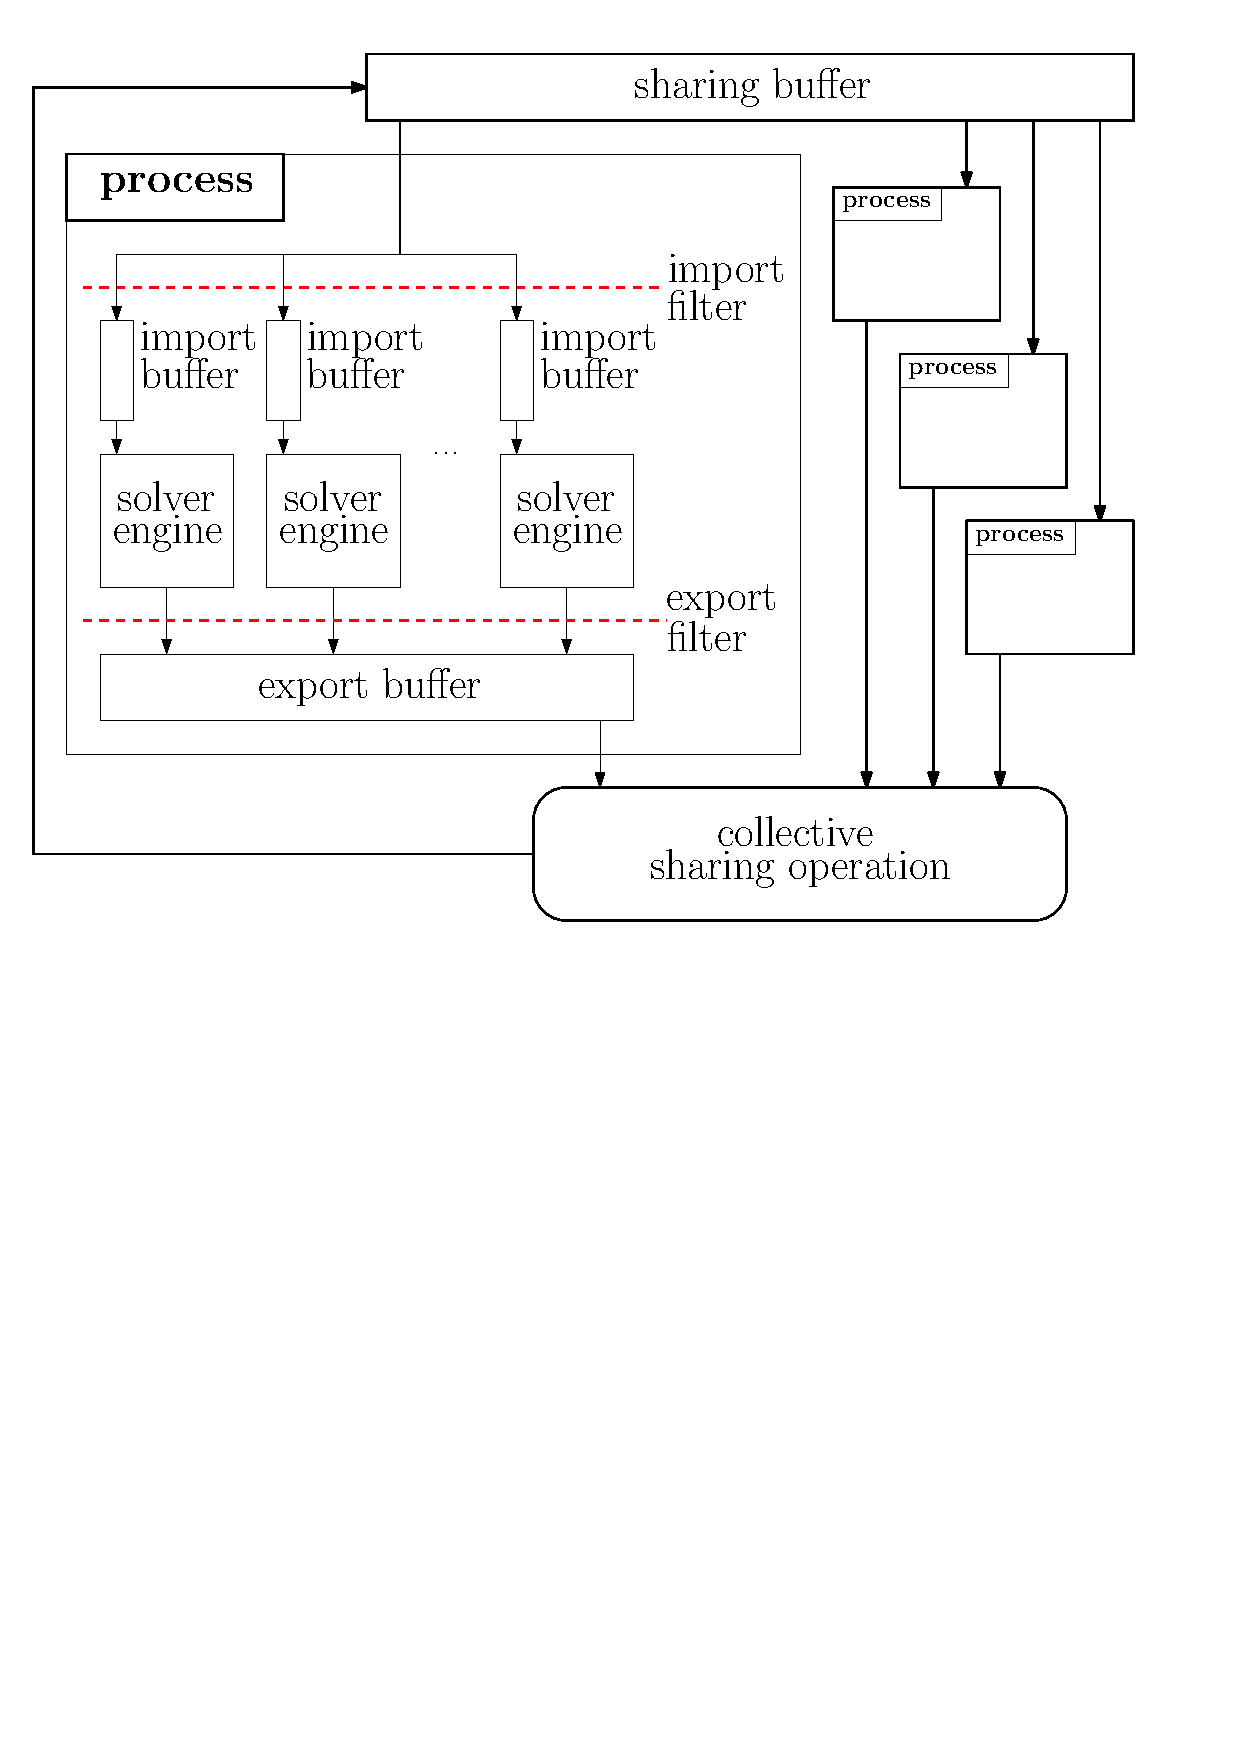
\includegraphics[scale=.8]{figures/mallob_architecture.pdf}
  \caption{MallobSat's process architecture. Arrows depict clause transfers. This depiction is inspired by Schreiber and Sanders' original depiction \cite{mallobSat}.}
  \label{fig:architectureMallob}
\end{figure}

MallobSat equips each process with a fixed maximum size import buffer for each of the processes solver engines and a single fixed maximum size export buffer that is shared between all solver engines in a process. The processes are organized into a distributed binary tree to enable clause sharing for distributed systems. The exchange of clauses between processes happens periodically. In the terminology of MallobSat the times between these so-called 'collective sharing operations' are called epochs. At the beginning of each epoch a collective sharing operation is executed: Each process merges its own export buffer with those of its children, filtering duplicate clauses along the way. This process is applied from the leaves up to the root of the binary communication tree. If the merged export buffer exceeds its limit, clauses are discarded by their priority. MallobSat prioritizes clauses first by length, then by their lbd value and finally lexicographically as a tie breaker. The export buffer's limit is sub-liniear in the sice of its current sub-tree, resulting in an increasing quality criterion up the tree. If the root process has recieved the merged export buffers, the resulting collection of clauses is then broadcast down the binary tree.

Clause sharing from the perspective of a solver engine inside a process happens asynchronously: If a solver engine has deduced a clause it sees fit to be shared, the engine simply executes a callback method provided by MallobSat at any time. If a a solver engine is ready to import external clauses (usually when restarting) it can iterate through its dedicated import buffer and import clauses from there. Usually an engine then has to do some filtering of its own, e.g. not to import clauses containing literals the engine already eliminated. Engines also need to shorten clauses even more, if it already falsified some literals contained in the newly imported clause.

To keep the communication volume as low as possible and to ensure important clauses are not lost to overflowing buffers, MallobSat employs some highly sophisticated filtering mechanisms for clauses that are imported and exported by solver engines. In particular these mechanisms prevent clauses from being mirrored back to the solver engine that produced them. They also prevent clauses from being imported by a solver engine multiple times, by filtering out any clauses that entered a solver engine's import buffer in the last $z$ epochs. The parameter $z$ is user-defined. Clauses are not indefinitely kept from being imported multiple times, since solvers tend to "forget" clauses regularly. This allows solver engines relearn important clauses after some time. We treat these filter mechanisms as blackboxes going forward. Like we mentiond earlier in this section, the interested reader is referred to the detailed description by Schreiber and Sanders in their dedicated article \cite{mallobSat}.

\subsubsection{Memory Efficient SAT-Solving}

Most research in SAT solving focuses on optimizing a solver's runtime for general-purpose SAT solving or specific use cases. With all the advancements over the past years, especially in parallel SAT solving, it has become feasible to solve ever more complex SAT problems and larger instances. However, this progress brings us to a point, where the memory consumption of a solver might become a bottleneck for its performance. Clause sharing portfolio solvers typically have their solver engines manage their clauses independently -- thus storing multiple copies of their clauses. Currently, there is little research on this frontier, other than pre- and inprocessing techniques reducing a CNF's size. Iser et al. addressed this problem, by adapting the portfolio solver Candy, to utilize a shared clause database \cite{iser2019memory}. Fleury and Biere approached the problem with their solver Gimsatul \cite{gimsatul}, by sharing clauses using a true shared memory approach -- storing only a single copy for every clause and merely exchanging pointers to clauses. Since Gimsatul is of particular interest to this work, we describe it in more detail below. Gimsatul's shared memory architecture makes it inherently unsuitable to be executed in distributed environments such as HPC-clusters, however. Iser et al. also evaluated their approach on only up to 16 cores, leaving massively parallel applications out of the question.

TODO: compression of cnfs

\subsubsection{Gimsatul}

Gimsatul \cite{gimsatul} is a parallel portfolio SAT solver that aims to reduce its memory consumption and enable aggressive clause sharing by using a shared memory approach for its clauses. The solver engines are CDCL solvers. In the terminology of Gimsatul these solver threads are called rings. There also exists a ruler thread, handling initialization and synchronization of its rings.

Gimsatul achieves its shared memory approach for clauses by only sharing pointers to newly derived clauses instead of whole clauses. To make this possible Fleury and Biere revisit the classical watcher data structures, resulting in all rings sharing their clauses in memory but maintaining their own watcher data structures independently. Further details are given in the original article \cite{gimsatul}.

We do want to describe Gimsatul's clause sharing mechanisms in more detail however, since this will become important later on. The process is depicted in Figure \ref{fig:architectureGimsatul}. If a ring derives a clause it deems worthy to share (i.e., a clause with a low glucose level) it will store a reference to this clause inside a buffer of small constant size for each other ring. If a buffer is full, it will overwrite the clause with the highest glucose level in the buffer. If all clauses in the buffer have a lower glucose level than the currently exported clause, it will not be inserted. When a ring decides to import a clause, it will pick another ring at random and import the clause with the lowest glucose level in it's respective buffer -- Deleting the clause from the buffer in the process.

\begin{figure}
  \center
  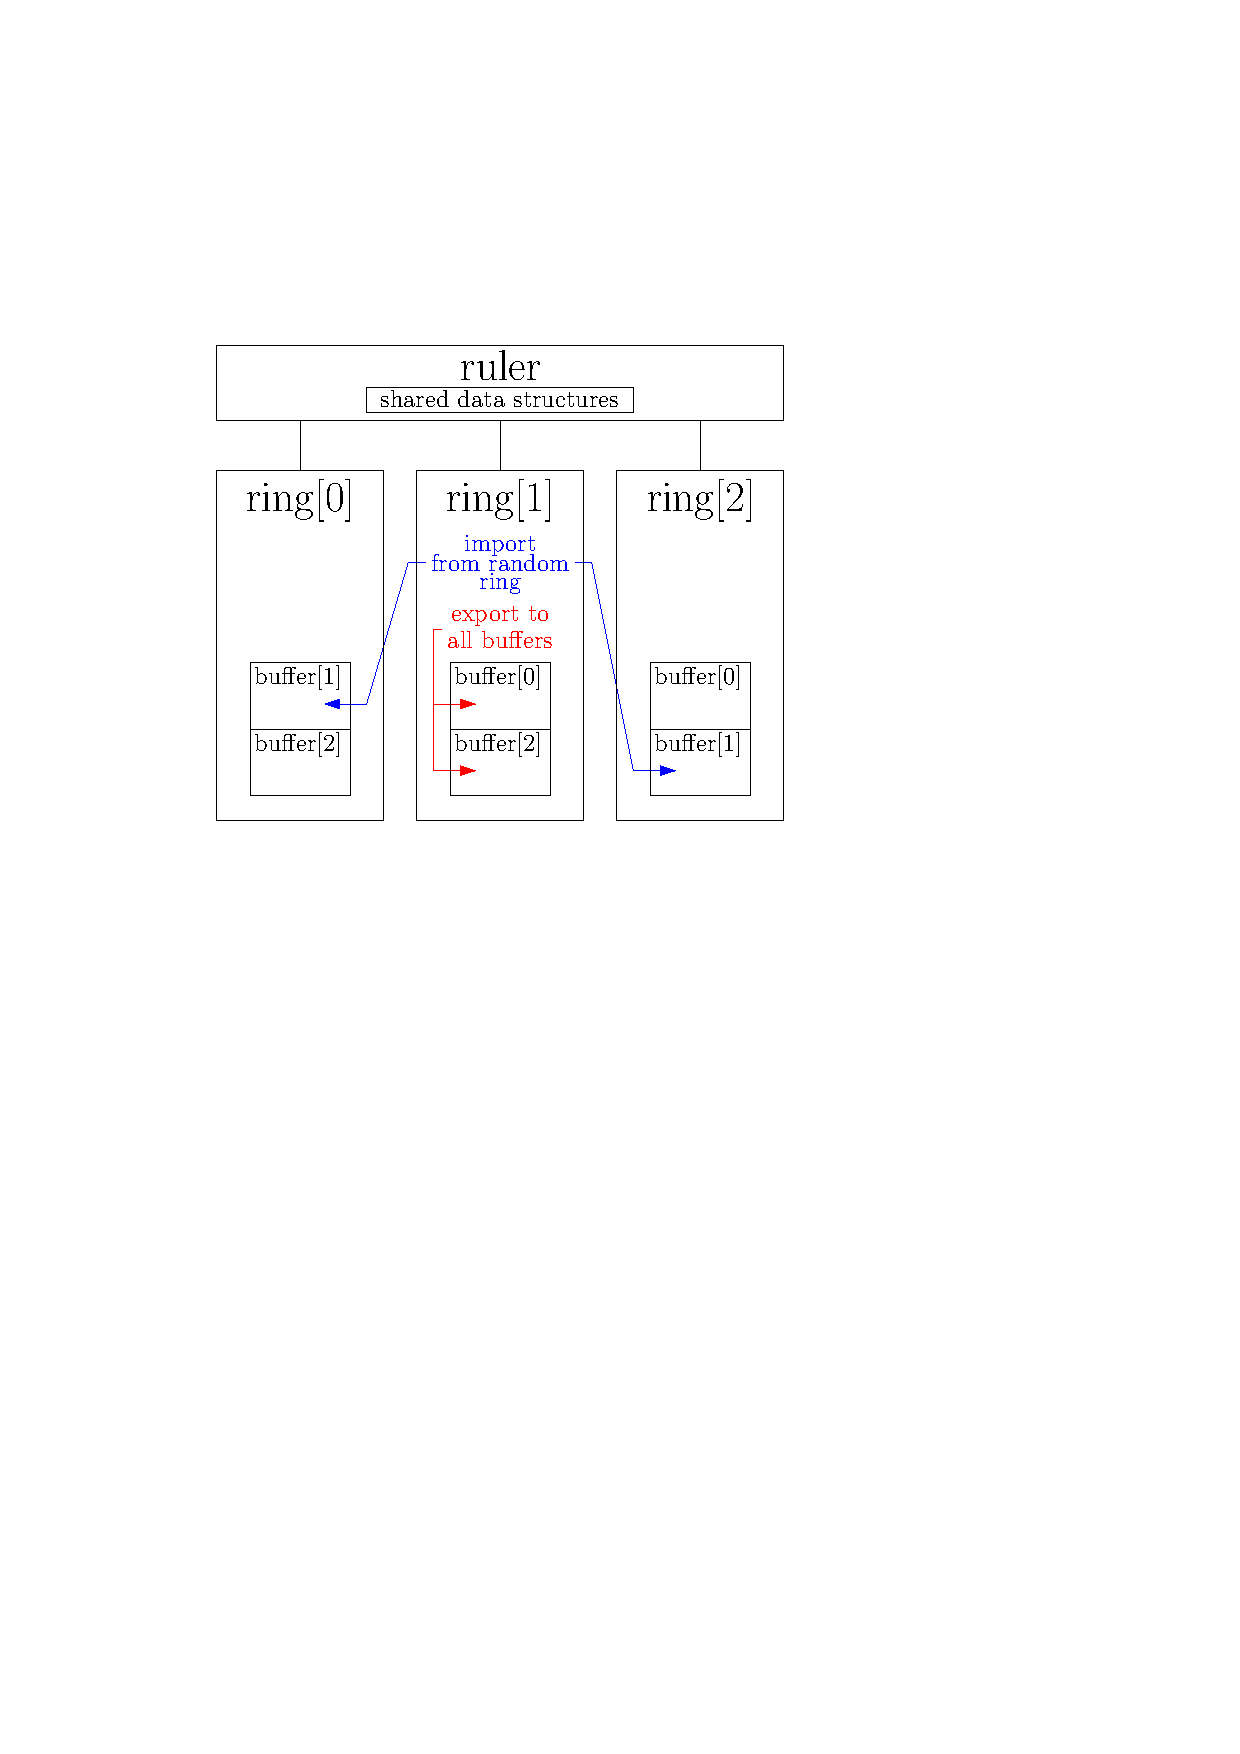
\includegraphics[]{figures/gimsatul_architecture.pdf}
  \caption{Gimsatul's clause sharing architecture for an examplary instance with 3 rings. This depiction is inspired by Fleury and Biere's original depiction \cite{gimsatul}.}
  \label{fig:architectureGimsatul}
\end{figure}

To diversify the rings, Gimsatul utilizes differing strategies for the first local search of each ring. A strategy consits of the restart strategy, the initial phases and whether or not reason bumping is activated. Possible restart strategies are \textit{focused mode}, \textit{stable mode} or a combination of the two as described by Biere and Fleury \cite{restartStrategy}. Initial phases are set either to 1 or 0 for all variables and reason bumping is either activated or deactivated. This results in up to 12 differing strategies. Again more detail is given in the original article \cite{gimsatul}.

%%%%%%%%%%%%%%%%%%%%%%%%%%%%%%%%%%%%%%%%%%%%%%%%%%%%%%%%%%%%%%%%%%%%%%

\section{Approach}

In this section we want to introduce MallobSat and Gimsatul, the core building blocks of our work. We integrated Gimsatul into MallobSat as a Solver backend to utilize both Gimsatul's memory efficiency, achieved by shared memory clause sharing, and MallobSat's massively parallel scalability. We also want to describe the architecture we used to make it possible to use the already parallel SAT solver Gimsatul as a solver backend in MallobSat.

\subsection{General Architecture}

We now want to describe the architecture of our algorithm, integrating Gimsatul (with its memory efficient shared memory approach) as a solver engine into MallobSat. In the following, we will use 'external' and 'internal' when talking about our architecture w.r.t. MallobSat from the point of a Gimsatul instance. E.g., when rings of a Gimsatul instance exchange derived clauses, we will denote this as 'internal clause exchange', if a Gimsatul instance is exchanging clauses as a solver engine in MallobSat we will call this 'external clause exchange'.

The most intuitive approach to integrate Gimsatul into MallobSat would be to consider each ring in a Gimsatul instance as a solver engine in MallobSat, complying with MallobSat's paradigm of each solver engine being a single SAT-solving thread. This approach runs into some fundamental problems however: 
First off, Gimsatul is initialized by reading the original CNF Formula of a given Problem, running some preprocessing, initializing a single ring and then cloning said ring $t - 1$ times to create its $t$ solving threads (i.e., rings). If we integrated each ring to be a solver engine in MallobSat, we would have to reimplement all of Gimsatul's initialization to create each ring independently. This would make it unfeasible to keep Gimsatul's shared memory clauses. Additionally MallobSat's clause sharing operation would double Gimsatul's internal clause sharing mechanisms -- potentially filtering important clauses from other other solver engines in favor of already internally shared clauses from the same Gimsatul instance.

For the aforementioned reasons we decided to implement a preferable architecture, shown in Figure \ref{fig:architecture}: We adapted Gimsatul to be a single solver engine in MallobSat, thus avoiding the initialization problems with Gimsatul. Furthermore, MallobSat's clause sharing and filtering avoid mirroring clauses to the solver engine they originate from -- thereby elegantly preventing redundant clause sharing between rings of the same Gimsatul instance.

\begin{figure}
  \center
  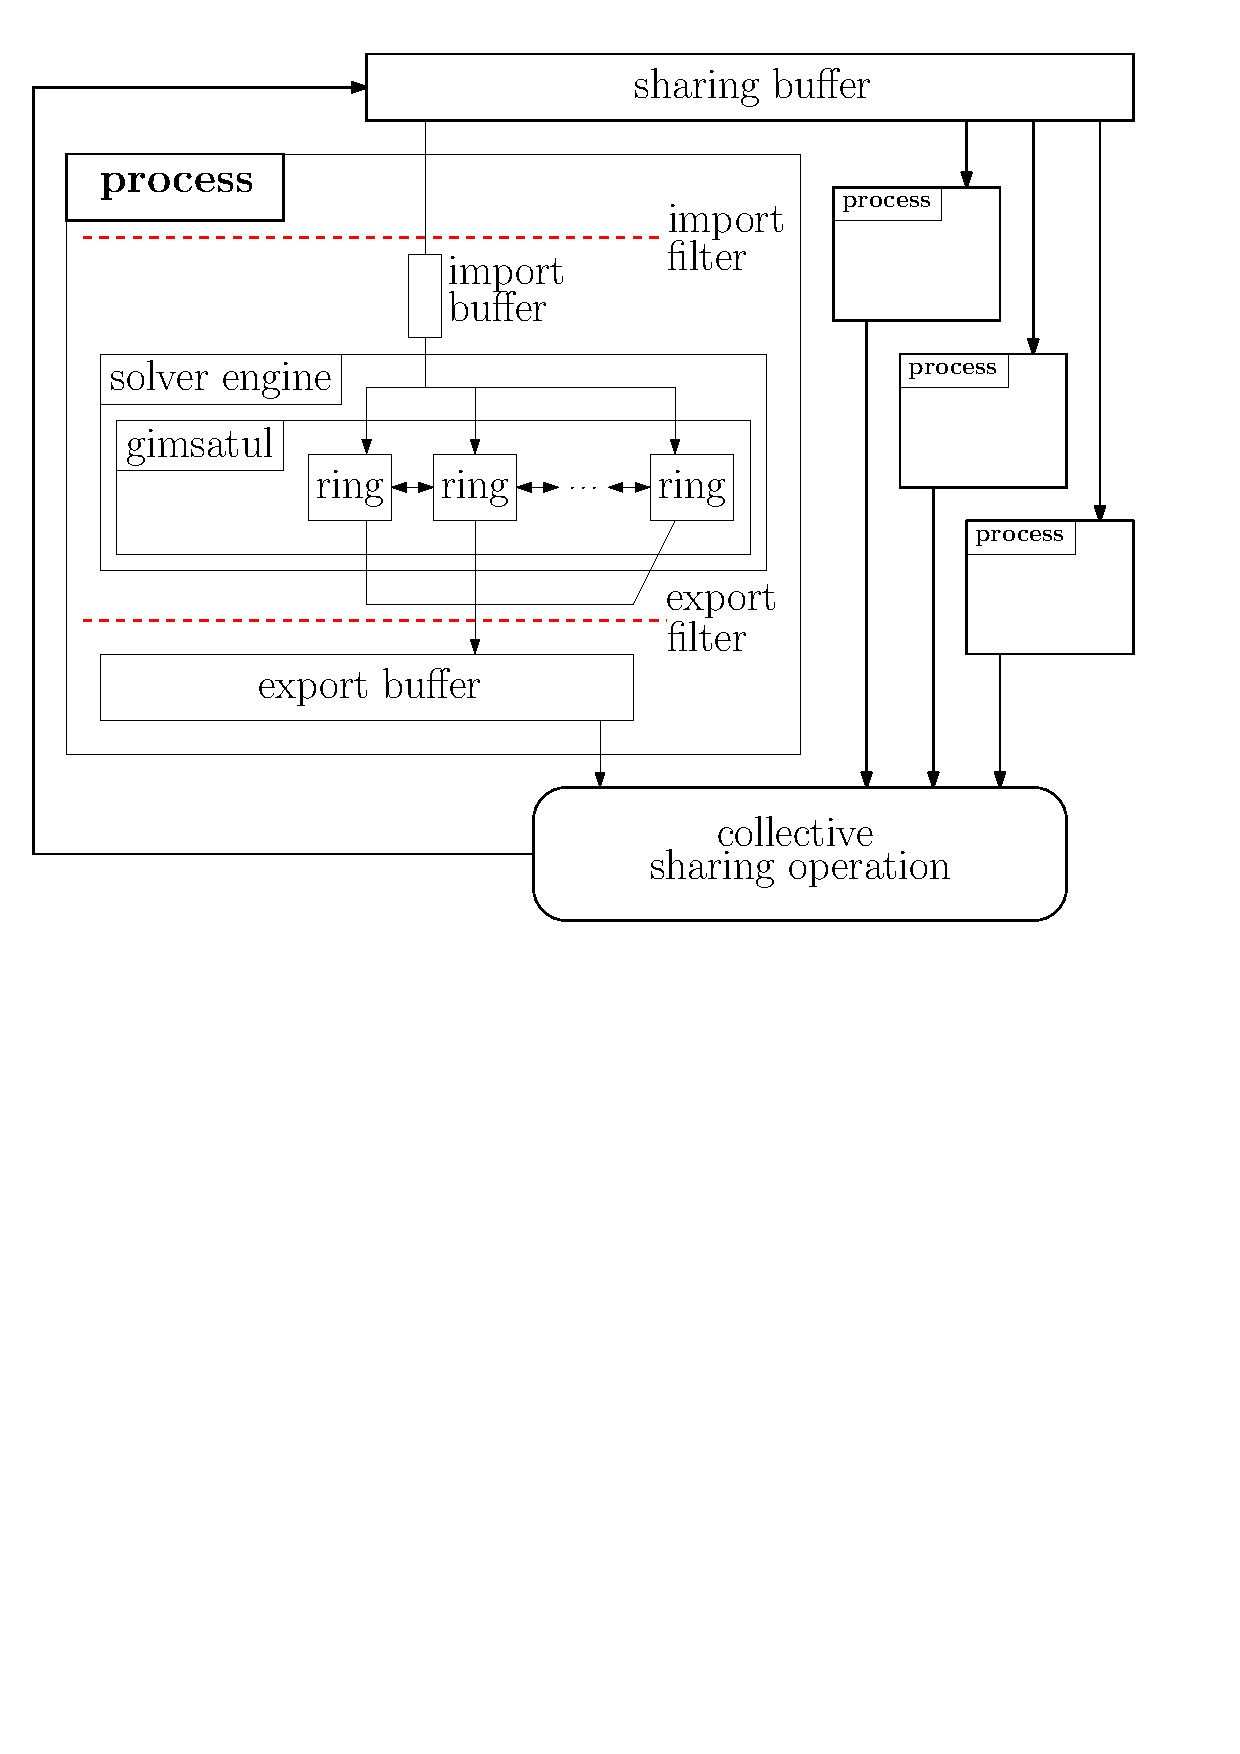
\includegraphics[scale=.8]{figures/architecture.pdf}
  \caption{Architecture integrating Gimsatul into MallobSat as a solver engine. Arrows depict clause transfers (or the transfer of references between rings).}
  \label{fig:architecture}
\end{figure}

\subsection{Creating the Solver Engine}

MallobSat assumes its solver engines to be serial blackbox SAT solvers, leaving us to redesign its engine setup to adopt a muti-threaded Gimsatul instance as a solver engine as follows: 
When initializing a process with $t$ solver engines (i.e., threads), MallobSat creates a portfolio of $t$ solvers from a given regular expression that defines the portfolio for the execution of MallobSat. We adapted this procedure to accumulate all $t' \leq t$ threads that are defined to be Gimsatul threads into a single solver engine and then run Gimsatul with $t'$ threads. The MallobSat process now contains $t - t'$ solver engines and operates as if it ran with $t - t'$ threads -- at most one of them being a Gimsatul Instance.

MallobSat and Gimsatul both implement some diversification over their respective threads (i.e., solver engines / rings). Since Gimsatul runs multiple rings inside a single solver engine we also had to adapt both these procedures to work in tandem.
The biggest part of MallobSat's diversification that actually has to be supported by the solver engine and is not done on a meta level over multiple engines are the so-called 'sparse random variable phases', originally introduced by Balyo et al. \cite{hordeSat}. This procedure flips the phases of random literals in a solver engine with probability $1 / e$ for a run with $e$ engines in total. Each process runs this algorithm with $e = t \cdot p$, where $t$ denotes the number of engines in a process and $p$ denotes the number of processes. Since Gimsatul runs with multiple threads we cannot na\"ively flip its phases like we could with a serial solver engine. Instead of flipping the phases given by MallobSat our Gimsatul engine calculates and applies the sparse random variable phases for its $t'$ rings itself (i.e., flipping a phase with probability $1 / (t' \cdot p)$). If a process runs with a single Gimsatul engine this results in the same outcome.
Gimsatul's native diversification only ever applies the same phase for all its variables. We added the calculated sparse random variable phases on top of Gimsatul's diversification by flipping the respective initial phases of a ring.

\subsection{Clause Export}

To export clauses from Gimsatul we took the simplest possible approach by latching the MallobSat clause export to Gimsatul's native internal clause export\footnote{Since Gimsatul does not trigger its clause sharing routines when executed with a single thread, it will also only export its derived clauses to MallobSat when run with at least 2 threads. Since our focus is on memory efficiency we do not see any reasons to run Gimsatul with a single thread and therefore do not consider this a problem.}. The reasoning being that if Gimsatul considers a clause to be good enough to be shared internally it is good enough to be shared externally through MallobSat. This might not always be the case however, since Gimsatul is sharing clauses fairly aggressively -- capitalizing on its shared memory approach to not have to copy the shared clauses on each export. Rather than implementing additional heuristics to differentiate between clauses that should be exported to other rings only and clauses that should be shared globally through MallobSat we decided to rely on MallobSat's sophisticated clause filtering. Thus incidentally saving on the additional execution time a complementary heuristic would entail.

Since MallobSat sees Gimsatul as a single solver engine it naturally keeps track of all the rings' clauses as being produced by a single thread, preventing redundant clause sharing through Gimsatul and MallobSat.

\subsection{Clause Import}

Usually MallobSat's solver engines import all the external clauses stored in their import buffer every time they do a restart. This way they are importing on decision level zero and do not have to consider their current state when deciding whether to keep the imported clauses. 

Importing external clauses into Gimsatul turned out to be a bit more complex though. Since we integrated Gimsatul as a single solver engine into MallobSat, we had to work with a single import buffer. MallobSat's import buffers are built in a way that clauses are immediately deleted when read by the solver engine. We want to reason our approach by first discussing two scrapped approaches.

\subsubsection{Rings Import Independently}

To make it possible for every ring to read the import buffer independently we would have had to redesign both MallobSat's import buffers, and Gimsatul's clause lifecycle. The import buffers would need some functionality to keep track of which rings had already read which clauses. And Gimsatul's rings would have needed some functionality to import only the reference to a clause, if it had already been imported into the shared memory by another ring. 

\subsubsection{Single dedicated importing ring.}
\label{sec:singleDedicatedImportRing}

Having a dedicated ring to import all clauses from the import buffer whenever it does a restart left the challenge of spreading the imported external clauses through all of Gimsatul's rings. This approach already resulted in some scalability improvements over vanilla Gimsatul. However, since Gimsatul's internal clause sharing utilizes buffers of extremely limited size, importing the full import buffer from MallobSat all at once, and immediately exporting them internally in Gimsatul, would discard many of the external due to internal buffer overflows.

\subsubsection{Our approach.}
\label{sec:ourApproach}

We combined the aforementioned approaches to spread externally imported clauses throughout Gimsatul's rings without having to import an external clause multiple times by letting each ring exclusively import a small set of clauses from MallobSat's import buffer: 
In our approach all rings try to import clauses from MallobSat's import buffer when restarting. To avoid race conditions and to minimize active waiting times we allow only one ring to import external clauses at a time. We utilize an atomic flag to indicate whether a ring is currently importing external clauses. If a ring is restarting and the flag is not set (i.e., no other ring is currently importing) it starts its importing routine. If the flag is set (i.e., some other ring is currently importing) it continues its solving routine to avoid actively waiting. 
When a ring is importing external clauses they are handled as if they were deduced by the importing ring and instantly internally exported to eventually spread them throughout all rings. Importing all available clauses in the import buffer, regularly leads to overflowing Gimsatul's internal buffers, as discussed in the section \ref{sec:singleDedicatedImportRing} above. To avoid this we propose the following 5 upper limits on the amount of clauses imported in one go.

\textbf{Minimum Free Slots.} Before importing external clauses, a ring checks all its internal export buffers, to find the one with the fewest free slots. This minimum is then used as the limit on importing external clauses.
This strategy does not result in the loss of any external clauses through overflowing buffers. It can, however, result in external clauses not being imported at all in this importing call, if at least one internal export buffer is full.
%To avoid overflowing Gimsatul's internal export buffers, it only ever imports at most a small constant number of clauses at once.
%a ring checks all of said export buffers for free slots before importing. It then only imports at most so many external clauses, that no overflows occur. For example: If we run a Gimsatul instance with 3 rings as a solver engine in MallobSat and ring 0 tries to import some external clauses it will check its export buffers for ring 1 and 2 and might find them to have 4 and 6 free slots respectively. It will then import at most 4 clauses from MallobSat's import buffer.

\textbf{Secondary Minimum Free Slots.} Like the first strategy, a ring will check all its internal export buffers. It will however, take the second to fewest free slots as the limit for importing external clauses. This strategy avoids a single full buffer from blocking the import operation.

\textbf{Mean Free Slots.} Before importing external clauses, a ring calculates the mean free slots over all its internal export buffers. This mean is then used as the limit on importing external clauses.
This strategy can result in not every external clause reaching every ring. We do expect external clauses to be imported more aggressively, however. Resulting in external clauses reaching rings earlier and sometimes replacing worse internal clauses in the internal export buffers.

\textbf{Amount of Rings.} The amount of rings in a Gimsatul instance is used as the limit on importing external clauses.
This follows the thought of ``one clause for every ring''. Since Gimsatul's internal export buffers are of limited constant size this results in overflowing buffers if there are too many rings in a single Gimsatul instance.

\textbf{Constant.} The limit is set by a small constant number between 1 and the size of the internal export buffers.

In our experiments we found the three strategies \textit{Mean Free Slots}, \textit{Amount of Rings} and \textit{Constant} to perform similarly and the remaining two strategies \textit{Minimum Free Slots} and \textit{Secondary Minimum Free Slots} notably worse.

%%%%%%%%%%%%%%%%%%%%%%%%%%%%%%%%%%%%%%%%%%%%%%%%%%%%%%%%%%%%%%%%%%%%%%

\section{Experimental Evaluation}

In this section, we want to discuss the findings of the experimental results of our approach. All experiments in this section were conducted on the SuperMUC-NG cluster at the \textit{Leibniz-Rechenzentrum} \cite{superMUC}. It is equipped with Intel Skylake Xeon Platinum 8174 processors clocked at 2.7 GHz. We evaluated our approach on up to 16 of the SuperMUC-NG's thin nodes, each containing 48 cores (96 hardware threads) with 96 GB memory. The SuperMUC-NG cluster runs on SUSE Linux (SLES) and connects its nodes via OmniPath \cite{omniPath}.

\subsection{Benchmarks}
To evaluate our algorithm, we used benchmark instances provided by Iser and Jabs on their Global Benchmark Database \cite{benchmarkDB}. Specifically, we used the 400 instances contained in the track \textit{main\_2024}, which was used in the 2024 SAT Competition \cite{satComp2024}. It is comprised of a myriad of different problems encoded as SAT instances.

\subsection{Configuration}
We ran our approach with one Gimsatul instance per node, i.e., 48 threads in one shared memory instance. Running multiple Gimsatul instances on the same node proved to yield comparable, or worse, results to only a single instance per node -- with a significant increase in memory costs. Using the node's capability of hyperthreading to exploit all 96 hardware threads in a single Gimsatul instance was not supported by MallobSat on the SuperMUC-NG cluster. We would not expect an increase in performance in this case regardless. In all cases, the configurations utilizing all 96 hardware threads performed worse than their counterparts, utilizing only the 48 cores. Figure \ref{fig:1nodeConfigCompare} shows our results for all the thread configurations we tested on one node. To save on computing time, we reason that the best configuration for a single node will also perform the best across multiple nodes. To reinforce this argument, we ran the best two configurations for one node on 2 compute nodes, as shown in Figure \ref{fig:2nodeConfigCompare}. In the following, we will denote the two configurations as follows:
\begin{itemize}
  \item[$A$:] 1 Gimsatul instance with 48 threads per node
  \item[$B$:] 2 Gimsatul instances with 24 threads each per node
\end{itemize}

In our experiments, configuration $B$ solved 10 benchmark instances that configuration $A$ did not solve within a $300\,$s time limit. Of these 10 instances, 7 were satisfiable, and thus some of them may be attributed to lucky non-determinism. Configuration $A$ solved 5 instances that configuration $B$ could not solve within the time limit. Of these 5 instances, 3 were satisfiable. We opted for the configuration $A$ regardless -- mainly due to its significantly reduced memory consumption as shown in Figure \ref{fig:2nodeConfigMemCompare}.

\begin{figure}
  \center
  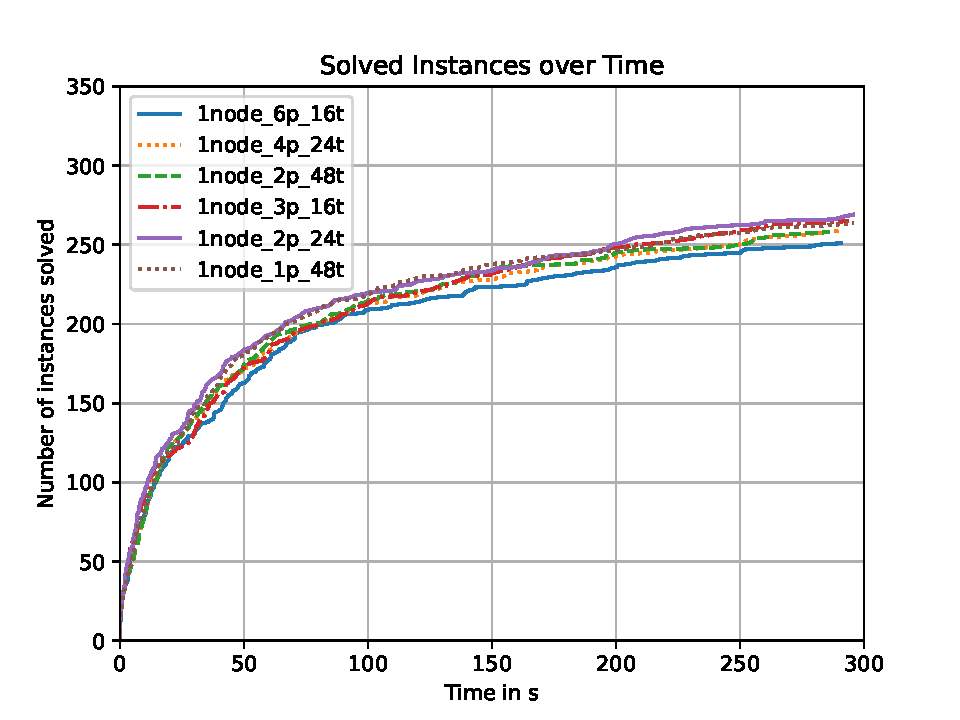
\includegraphics[scale=.5]{plots/config_compare/1node_config_compare.pdf}
  \caption{Comparison between thread configurations on a single node.}
  \label{fig:1nodeConfigCompare}
\end{figure}

\begin{figure}
  \center
  \begin{subfigure}[c]{0.45\textwidth}
    \center
    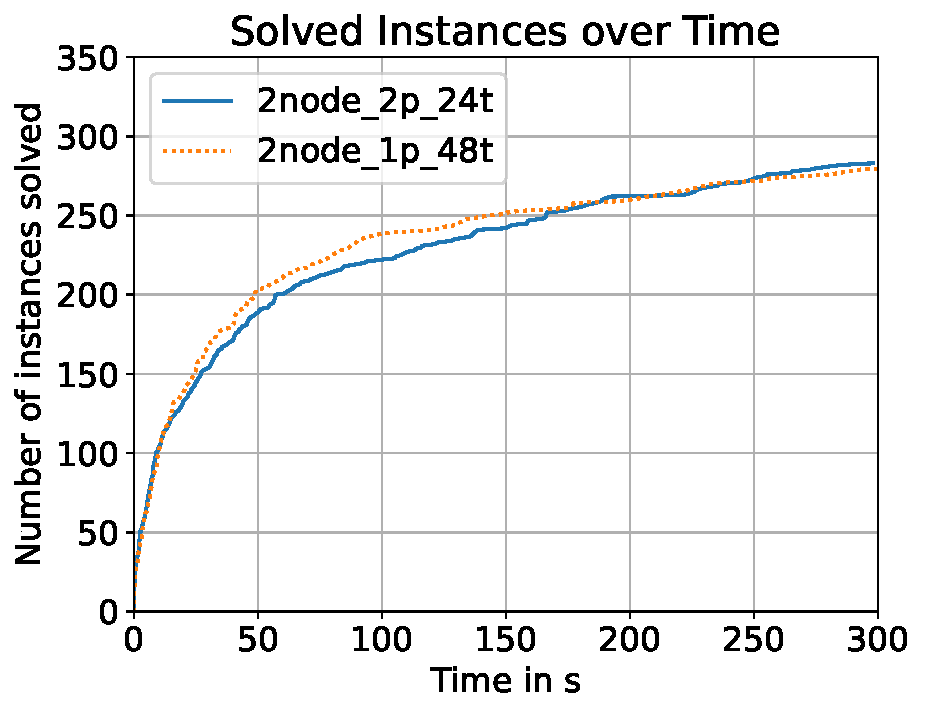
\includegraphics[scale=0.45]{plots/config_compare/2node_config_compare.pdf}
    \caption{}
    \label{2nodeConfigRuntimeCompare}
  \end{subfigure}
  \hfill
  \begin{subfigure}[c]{0.45\textwidth}
    \center
    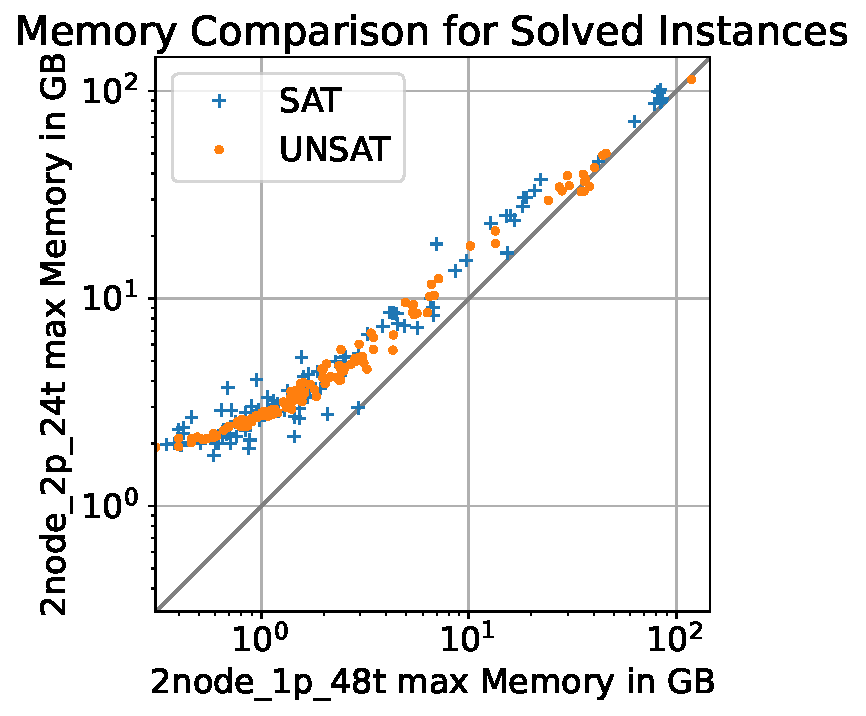
\includegraphics[scale=0.45]{plots/config_compare/2node_config_mem_compare.pdf}
    \caption{}
    \label{fig:2nodeConfigMemCompare}
  \end{subfigure}
  \caption{Comparison between thread configurations on two nodes.}
  \label{fig:2nodeConfigCompare}
\end{figure}

To further configure MallobSat's options, we implemented a search-only approach with only a single preprocessor as introduced by Schreiber et al. \cite{searchOnlyPaper}. To do this, we deactivated all pre- and inprocessing procedures in our Gimsatul instances, i.e., no simplification or probing. For Gimsatul this has the additional effect of avoiding synchronization between all rings of a Gimsatul instance. This increases memory consumption due to missing compacting procedures but avoids idling rings while waiting for other rings to synchronize. To preprocess the formula, we utilized the Kissat SAT solver \cite{kissat}. In preliminary experiments, we found a significant increase in performance due to this practice and therefore employ it throughout all of our experiments. As the import strategy (as discussed in Section \ref{sec:ourApproach}), we chose the \textit{Amount of Rings} strategy, since it performed best in testing.

\subsection{Runtime and Memory Usage}

First, we to discuss our findings on runtime with respect to scalability on up to 16 nodes (i.e., 768 cores). We then compare our approach to the state of the art distributed SAT solver MallobSat, using its default configuration utilizing one Kissat instance per core.

\subsubsection{Speedups}

As shown in Figure \ref{fig:runtimeCompareGim}, we ran our algorithm on 1, 2, 4, 8, and 16 nodes respectively. We can see an increase in performance with an increasing amount of available processing power, albeit with diminishing returns.

\begin{figure}
  \center
  \begin{subfigure}[c]{.45\textwidth}
    \center
    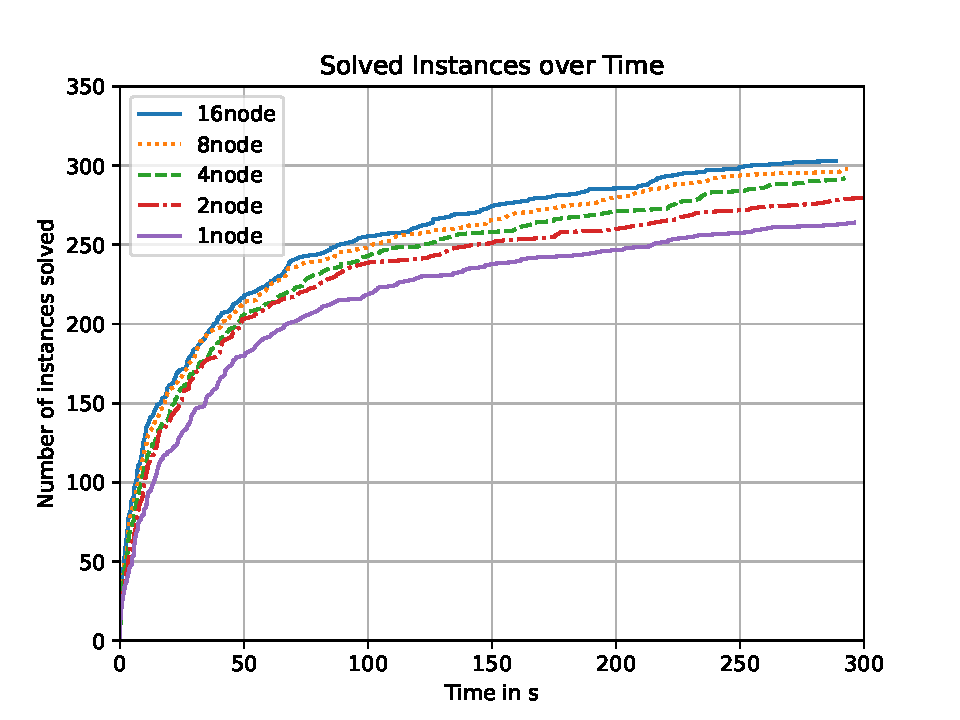
\includegraphics[scale=.45]{plots/cumulative_runtime/scalability_gim.pdf}
    \subcaption{Scalability of our approach}
    \label{fig:runtimeCompareGim}
  \end{subfigure}
  \hfill
  \begin{subfigure}[c]{.45\textwidth}
    \center
    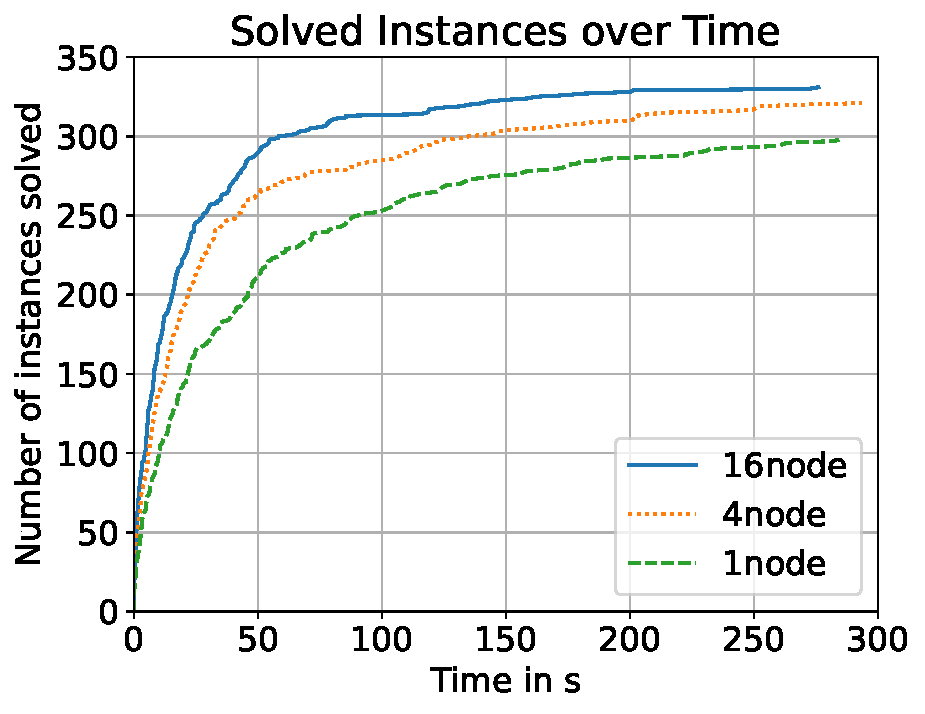
\includegraphics[scale=.45]{plots/cumulative_runtime/scalability_kis.pdf}
    \subcaption{Scalability of MallobSat}
    \label{fig:runtimeCompareKis}
  \end{subfigure}
  \caption{Scalability of our approach compared to MallobSat}
  \label{fig:scale}
\end{figure}

To calculate speedups, we ran the sate of the art serial SAT solver Kissat \cite{kissat} for up to 3000 s on a single core. The results of this run are shown in Figure \ref{fig:runtimeSerial}. The geometric means of all speedups for benchmark instances solved by Kissat are shown in Table \ref{tab:speedups}. For most families, we see an increase in the geometric mean speedup for our approach with increasing numbers of cores. The specific speedups, for all instances that were solved by Kissat within the 3000 s time limit, are shown in Figure \ref{fig:speedups}. Here we observe a significant variation in speedups for simple instances (i.e., instances Kissat solved in under 500 seconds). For complex instances (i.e., instances where Kissat needed more than 500 seconds), we see a tendency for the speedups to become greater. For very complex instances the speedups routinely beat the geometric mean while their variance increases even more.

\begin{figure}
  \center
  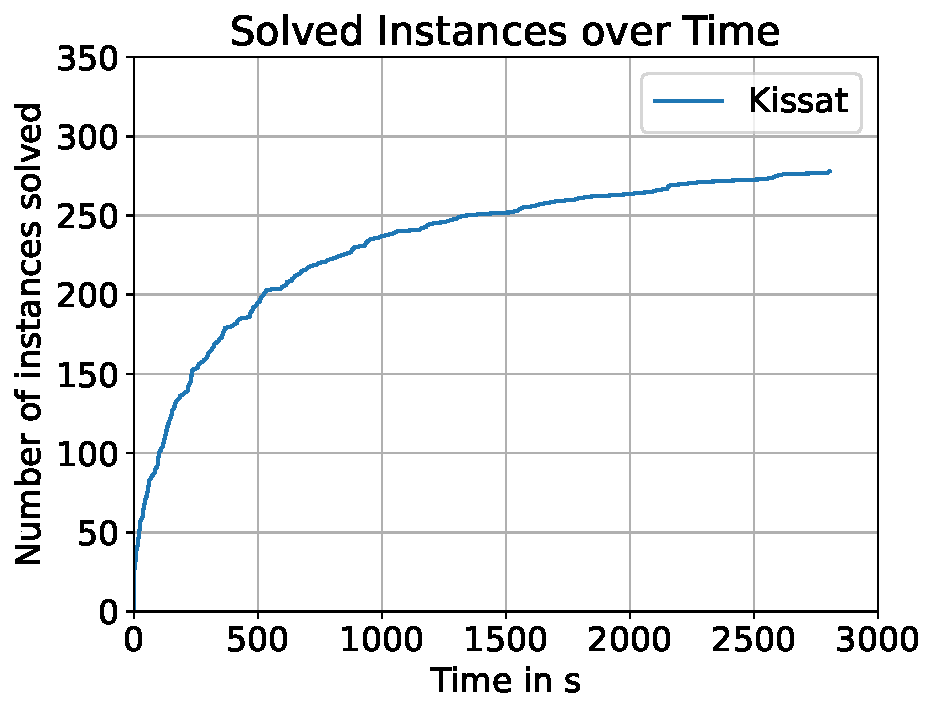
\includegraphics[scale=.5]{plots/cumulative_runtime/scalability_serial.pdf}
  \caption{Scalability of serial Kissat}
  \label{fig:runtimeSerial}
\end{figure}

\begin{table}
  \center
  \begin{tabular}{ cccc }
    \toprule
    \multicolumn{2}{c}{Setup} & \multicolumn{2}{c}{Solver}\\
    \#nodes   & \#cores   & Our Approach  & MallobSat \\
    \midrule
    1  & 48  & 5.357    & 7.847\\
    2  & 96  & 7.384    & -\\
    4  & 192 & 8.146    & 14.034\\
    8  & 384 & 9.720    & -\\
    16 & 762 & 10.260   & 20.073\\
    \bottomrule
  \end{tabular}
  \caption{Geometric mean speedups for number of processors}
  \label{tab:speedups}
\end{table}

\begin{figure}
  \center
  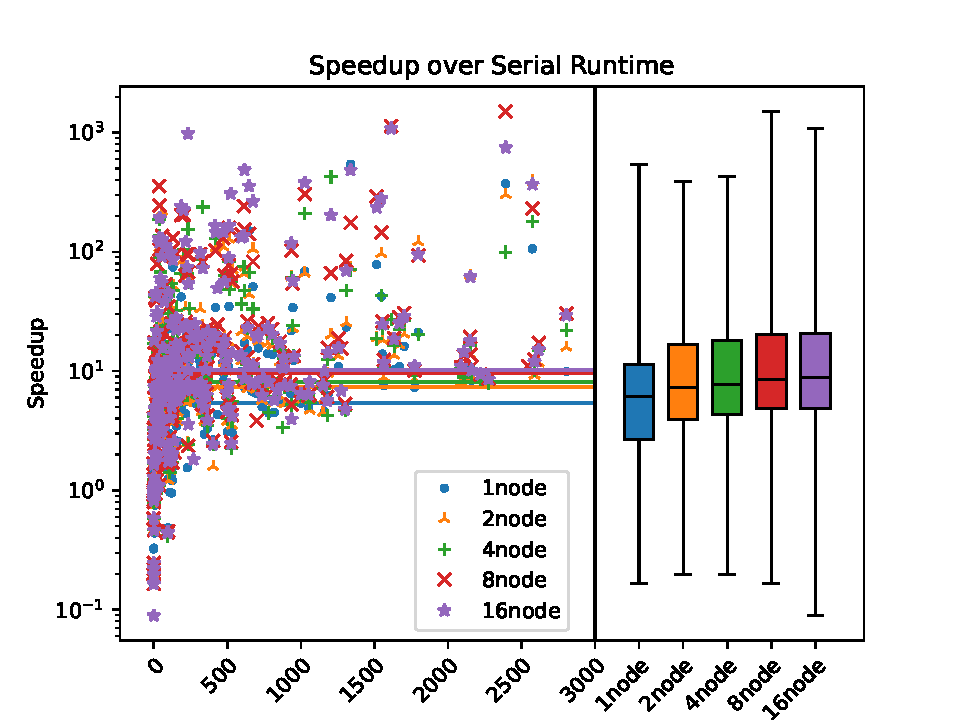
\includegraphics{plots/speedups_gim.pdf}
  \caption{Speedups of our Algorithm. Per instance on the left, accumulated on the right.}
  \label{fig:speedups}
\end{figure}

%%
% Speedup < 1:
%   cryptography-simon: 10/10   alle sat
%   heule-folkman: 3/11   alle sat
%   maxsat-optimum: 1/13
%   miter: 9/47
%   planning: 1/6 alle unsat
%   reg-n: 2/4 alle unsat
%   scheduling: 2/50
%   software-verification: 2/15 alle unsat
%   subgraph-isomorphism: 2/4   die beiden sat sind langsamer, die beiden unsat schneller

Table \ref{tab:speedupsSignificantFamilies} shows speedups separated by significant families. We consider families to be significant if at least five instances contained in our benchmark set belong to this family. A complete table of all instance families is provided in the Appendix \ref{app:speedupsFamiliesComplete}. We calculated the geometric mean speedups per family for all our configurations and ordered them by the geometric mean speedup over all 5 configurations.

For all instances of the family \textit{cryptography-simon}, we found our approach to be slower than serial Kissat. This might suggest a systematic incompatibility between our approach and this kind of problem. All instances of this family, however, were solved in under $0.01\,$s by Kissat. Since the fastest measured runtime of our approach is $0.03\,$s, we attribute any slowdown for instances below $0.03\,$s to our increased startup overhead compared to Kissat.

For instances of the family \textit{heule-folkman}, which encode proofs of whether a graph is a so-called Folkman Graph \cite{satComp2024}, we find that serial Kissat generally performs better than our approach. In our experiments, Kissat solved all 10 instances of this family in our benchmark set while our approach only solved at most 3 instances. We currently cannot give a specific reason for this phenomenon. Schreiber et al. \cite{searchOnlyPaper} found their search-only approach in MallobSat to be non-beneficial on this family of instances as well. We therefore conclude that some inprocessing techniques applied by Kissat result in significant improvements in this case. Since we deactivated all pre- and inprocessing to improve overall performance, our approach appears to be unsuitable for the \textit{heule-folkman} family.

We find the highest geometric mean speedups, for any significant family, for a family called \textit{rbsat}. Instances of this family have been part of multiple SAT competitions over the years. However, there is no specific information about this family available. All five instances in our benchmark set are satisfiable. Kissat was able to solve three of them within its time limit of 3000 seconds.

Instances of the family \textit{minimum-disagreement-parity} \cite{satComp2022}, encode the Minimum Disagreement Parity (MDP) problem, which is of interest to the cryptography community and results in challenging SAT problems. This is underlined by the small size of these instances: The largest one contains only 1021 variables, with the slowest solved by Kissat taking $2617.82\,$s and containing only 750 variables. This family comprises of 3 satisfiable, and 3 unsatisfiable instances. Our high geometric mean speedups of over 22 suggest that the MDP problem instances benefit from the increased processing power of parallel sat solving far more than other kinds of problems.

\begin{table}
  \center
  \begin{tabular}{ lcccccc }
    \toprule
    family	&	\#	&	1node	&	2node	&	4node	&	8node	&	16node\\
    \midrule
    coloring	&	8	&	-	&	-	&	-	&	-	&	-\\
    heule-folkman	&	11	&	0.425	&	-	&	0.416	&	0.449	&	0.444\\
    cryptography-simon	&	10	&	0.221	&	0.234	&	0.227	&	0.2	&	0.18\\
    miter	&	47	&	1.705	&	1.835	&	1.997	&	2.25	&	2.013\\
    random-circuits	&	15	&	2.598	&	3.095	&	3.527	&	3.849	&	3.839\\
    planning	&	6	&	2.567	&	3.977	&	4.168	&	4.623	&	4.835\\
    software-verification	&	15	&	2.564	&	5.073	&	4.248	&	4.57	&	4.71\\
    tseitin-formulas	&	8	&	4.442	&	4.567	&	5.177	&	5.275	&	5.49\\
    hardware-verification	&	5	&	4.621	&	5.369	&	5.556	&	6.036	&	6.161\\
    scheduling	&	50	&	5.333	&	6.434	&	7.944	&	8.384	&	8.799\\
    heule-nol	&	11	&	5.988	&	11.793	&	7.786	&	10.231	&	12.876\\
    cryptography-ascon	&	6	&	7.396	&	8.273	&	10.115	&	8.709	&	14.008\\
    maxsat-optimum	&	13	&	7.419	&	7.32	&	12.362	&	13.762	&	14.899\\
    quantum-kochen-specker	&	10	&	9.356	&	11.237	&	11.186	&	11.137	&	11.005\\
    cryptography	&	7	&	6.32	&	16.922	&	9.289	&	21.402	&	23.632\\
    hamiltonian	&	40	&	8.968	&	14.409	&	19.398	&	23.315	&	26.351\\
    argumentation	&	21	&	13.01	&	16.268	&	18.577	&	21.941	&	20.716\\
    independent-set	&	15	&	16.442	&	18.038	&	20.981	&	27.173	&	25.9\\
    minimum-disagreement-parity	&	17	&	40.311	&	22.119	&	24.766	&	46.884	&	58.316\\
    rbsat	&	5	&	47.606	&	64.654	&	76.039	&	186.204	&	221.286\\
    \bottomrule
  \end{tabular}
  \caption{Speedups per family and setup for families comprising at least 5 instances and a calculatable speedup.}
  \label{tab:speedupsSignificantFamilies}
\end{table}

\subsubsection{Comparison to MallobSat}
\label{sec:compare}

In the following, we denote benchmark instances that have been solved by all solvers in a given context as \textit{solved instances}. Conversely, we denote instances that have not been solved by at least one solver in a given context as \textit{unsolved or partially solved instances}.

Figure \ref{fig:runtimeCompare} shows the compared runtimes of solved instances for Mallob on the x-axis and our approach on the y-axis. We differentiate between satisfiable and unsatisfiable instances. While the satisfiable instances show a wider variance than the unsatisfiable ones, it is clear that our approach sacrifices runtime efficiency for memory efficiency. Especially for complex instances, we observe a clear tendency for our algorithm to take up to an order of magnitude more time.

\begin{figure}
  \center
  \begin{subfigure}[c]{.45\textwidth}
    \center
    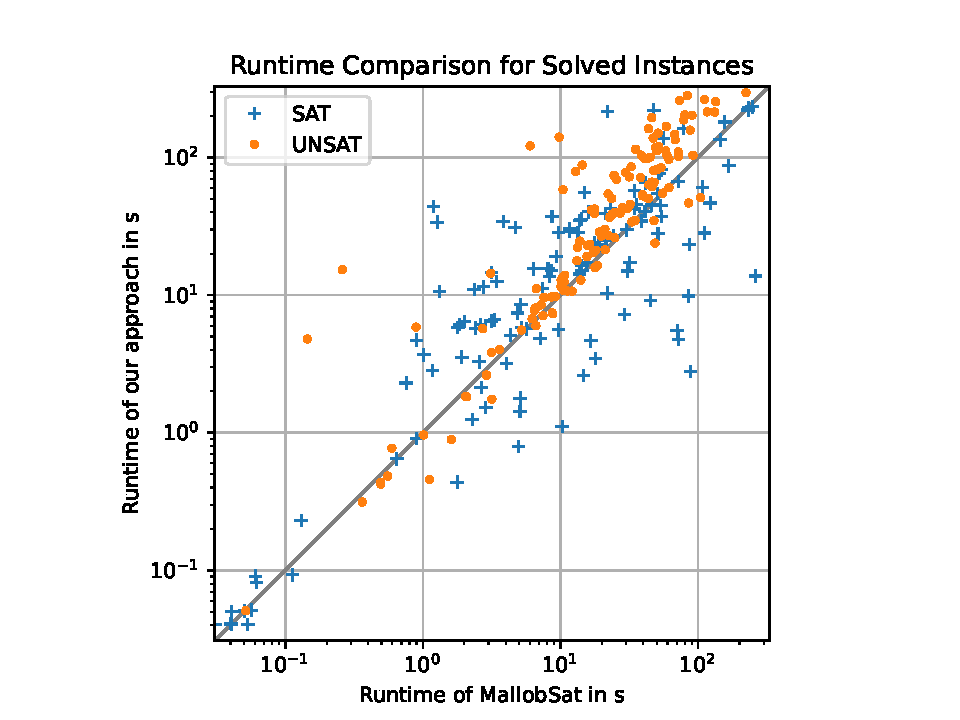
\includegraphics[scale=.45]{plots/square_runtime_compare/square_runtime_1node.pdf}
    \subcaption{1 node}
    \label{fig:runtimeCompare1node}
  \end{subfigure}
  \begin{subfigure}[c]{.45\textwidth}
    \center
    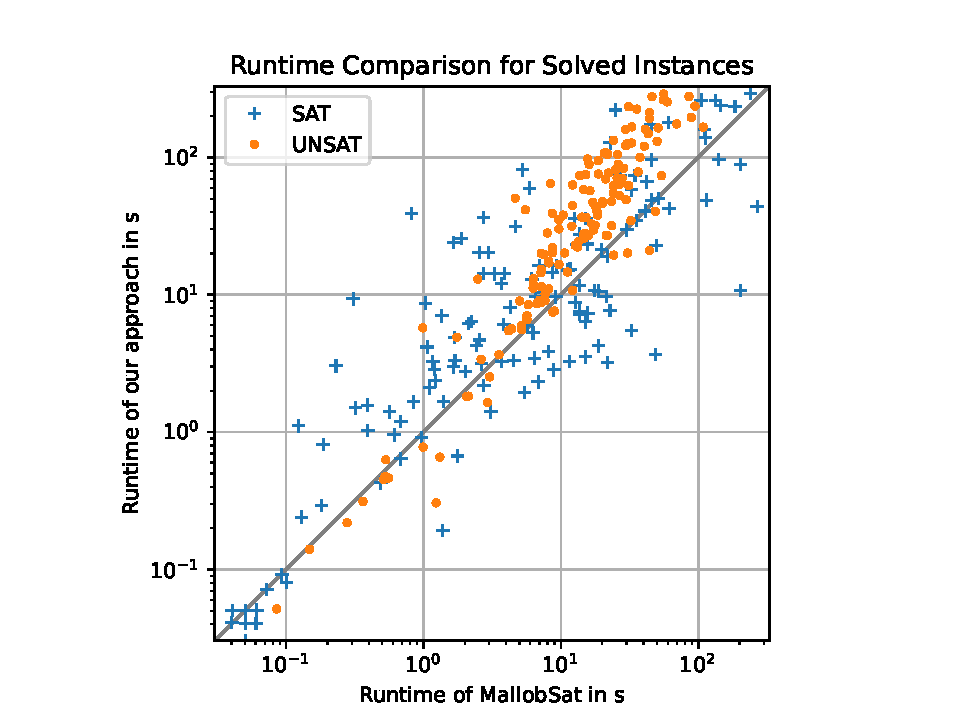
\includegraphics[scale=.45]{plots/square_runtime_compare/square_runtime_4node.pdf}
    \subcaption{4 nodes}
    \label{fig:runtimeCompare4node}
  \end{subfigure}
  \begin{subfigure}[c]{.45\textwidth}
    \center
    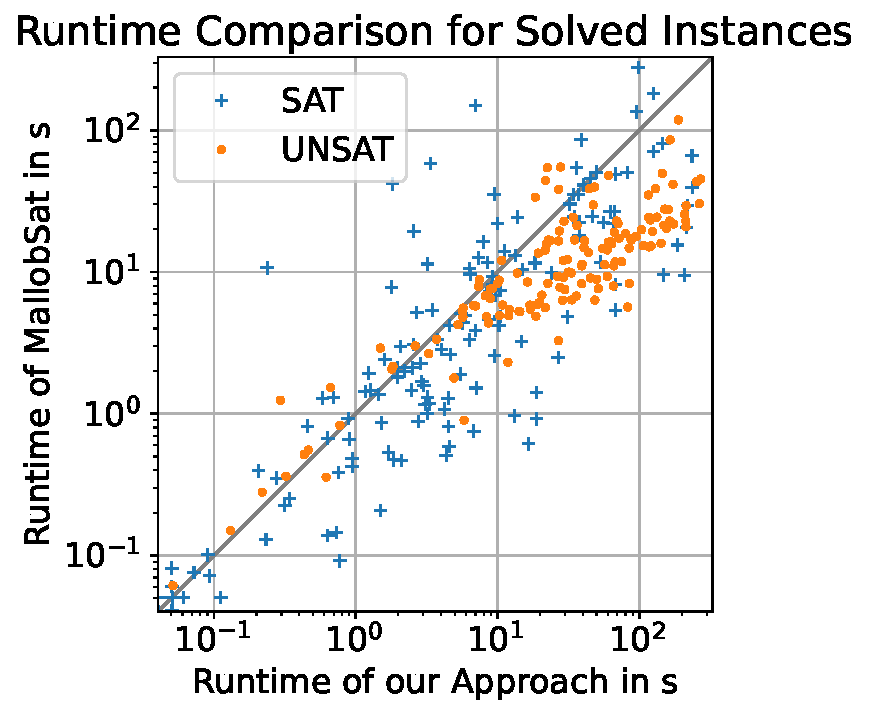
\includegraphics[scale=.45]{plots/square_runtime_compare/square_runtime_16node.pdf}
    \subcaption{16 nodes}
    \label{fig:runtimeCompare16node}
  \end{subfigure}
  \caption{Runtime Comparison between MallobSat and our approach.}
  \label{fig:runtimeCompare}
\end{figure}

Figure \ref{fig:memCompare} shows the comparison between our approach's and MallobSat's memory consumption in a similar manner: with MallobSat's peak memory consumption on the x-axis and the peak memory consumption of our approach on the y-axis. Again, we differentiate between satisfiable and unsatisfiable instances. Here, we clearly see our approach consuming less -- in extreme cases, more than an order of magnitude less -- memory than MallobSat.

\begin{figure}
  \center
  \begin{subfigure}[c]{.45\textwidth}
    \center
    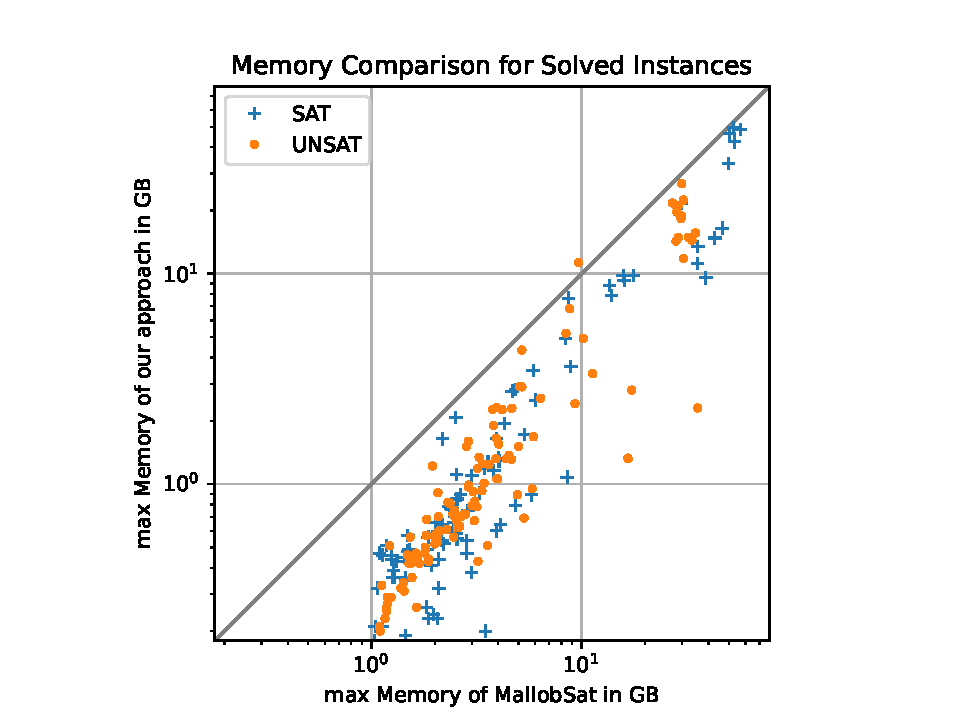
\includegraphics[scale=.45]{plots/square_mem_compare/square_mem_1node.pdf}
    \subcaption{1 node}
    \label{fig:memCompare1node}
  \end{subfigure}
  \begin{subfigure}[c]{.45\textwidth}
    \center
    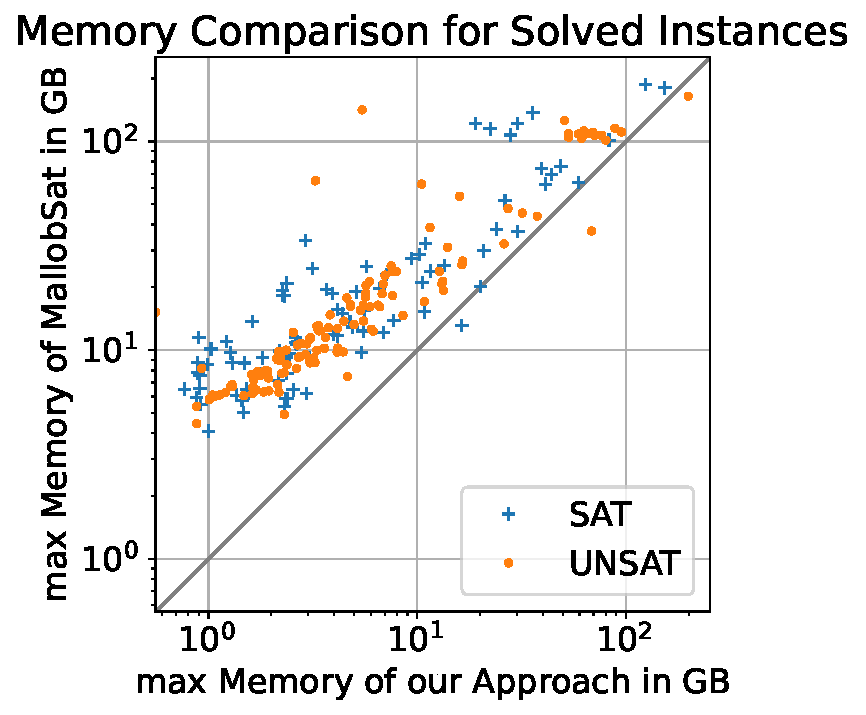
\includegraphics[scale=.45]{plots/square_mem_compare/square_mem_4node.pdf}
    \subcaption{4 nodes}
    \label{fig:memCompare4node}
  \end{subfigure}
  \begin{subfigure}[c]{.45\textwidth}
    \center
    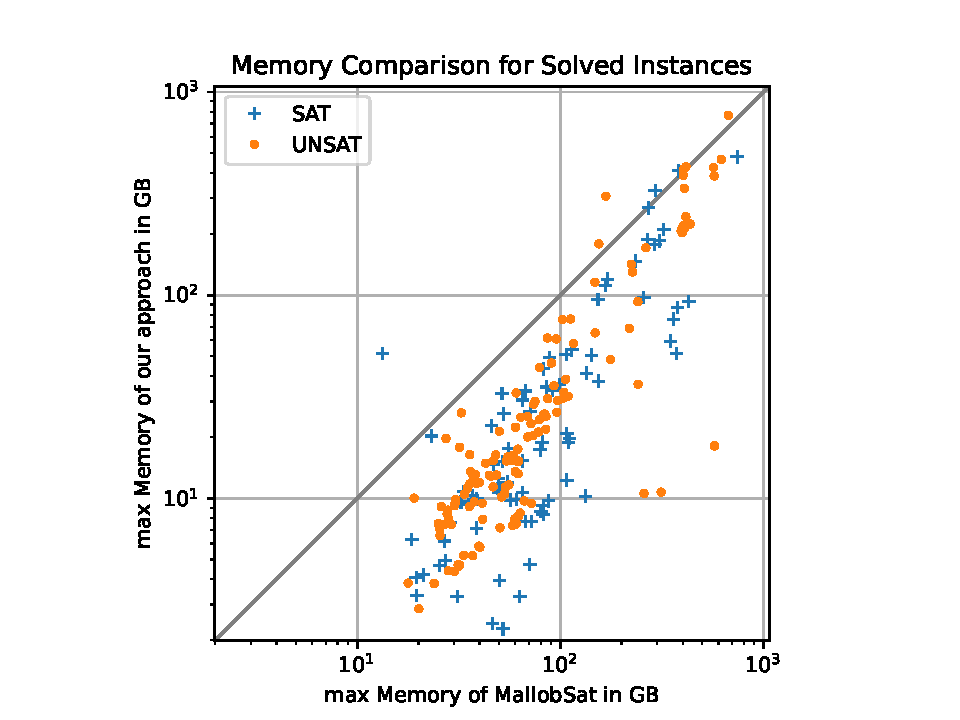
\includegraphics[scale=.45]{plots/square_mem_compare/square_mem_16node.pdf}
    \subcaption{16 nodes}
    \label{fig:memCompare16node}
  \end{subfigure}
  \caption{Memory Comparison between MallobSat and our approach.}
  \label{fig:memCompare}
\end{figure}

The exact memory consumption of our approach, as well as MallobSat's, is shown in Figure \ref{fig:memAbsVars}. The mean memory consumptions across all instances are shown in Table \ref{tab:memMean}. For solved instances, we find the ratio between MallobSat's mean memory consumption and that of our approach to be $1.836$ for 1 node, $1.881$ for 4 nodes, and $1.883$ for 16 nodes. For all instances, we find the ratios to be slightly smaller on multiple nodes: $1.893$ for 1 node, $1.655$ for 4 nodes, and $1.722$ for 16 nodes.

\begin{figure}
  \center
  \begin{subfigure}[c]{.45\textwidth}
    \center
    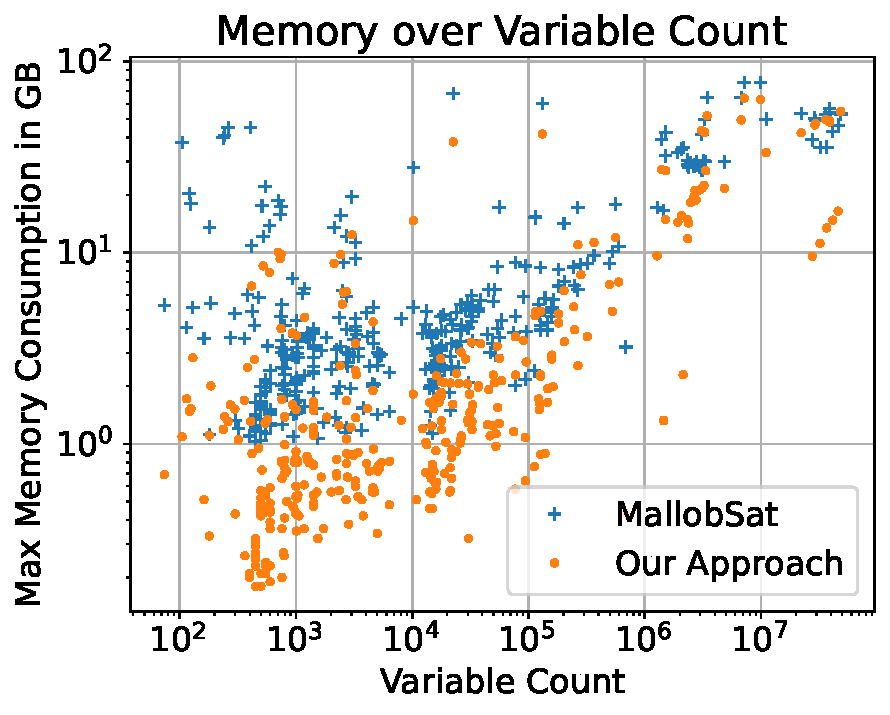
\includegraphics[scale=.45]{plots/1node_compare/mem_abs_over_vars.pdf}
    \caption{1 node}
  \end{subfigure}
  \begin{subfigure}[c]{.45\textwidth}
    \center
    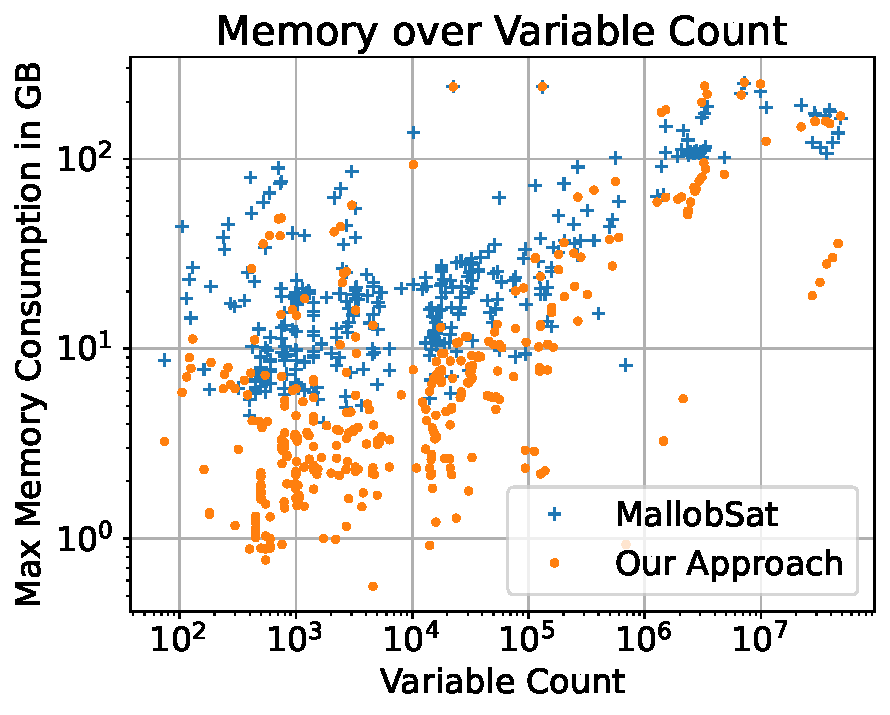
\includegraphics[scale=.45]{plots/4node_compare/mem_abs_over_vars.pdf}
    \caption{4 nodes}
  \end{subfigure}
  \begin{subfigure}[c]{.45\textwidth}
    \center
    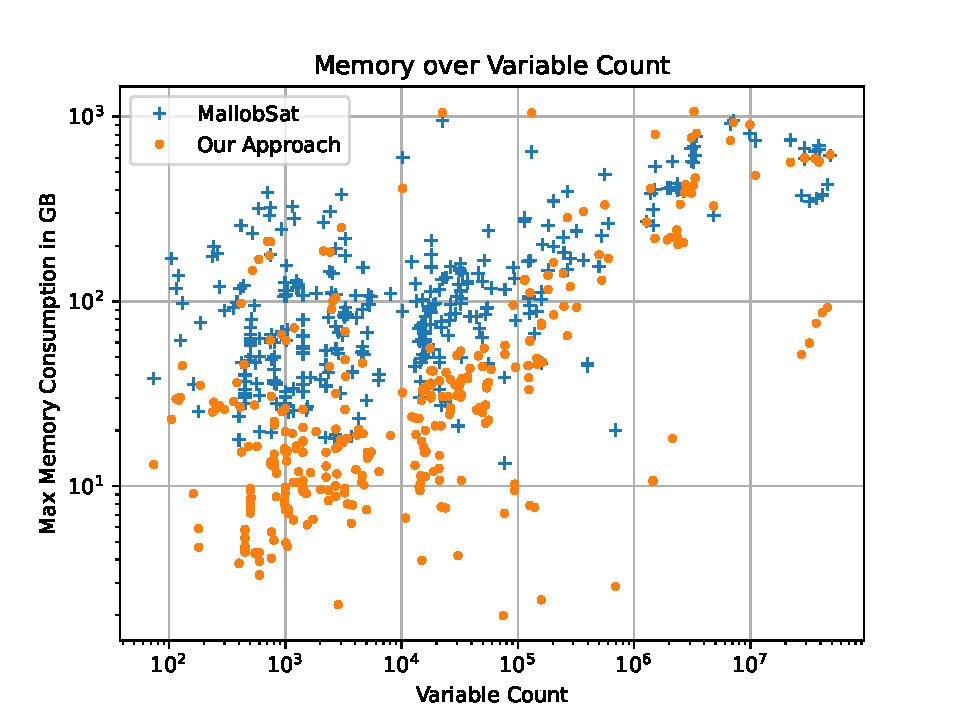
\includegraphics[scale=.45]{plots/16node_compare/mem_abs_over_vars.pdf}
    \caption{16 nodes}
  \end{subfigure}
  \caption{Memory consumption over variables.}
  \label{fig:memAbsVars}
\end{figure}

\begin{table}
  \center
  \begin{tabular}{ cccccc }
    \toprule
    \multicolumn{2}{c}{Setup} & \multicolumn{2}{c}{Solved Instances} & \multicolumn{2}{c}{All Instances}\\
    \#nodes & \#cores & Our Algorithm & MallobSat & Our Algorithm & MallobSat \\
    \midrule
    1  & 48  & 3.745  & 6.875   & 4.488   & 8.494\\
    2  & 96  & 7.159  & -       & 9.301   & -\\
    4  & 192 & 13.628 & 25.631  & 18.686  & 30.921\\
    8  & 384 & 27.357 & -       & 37.176  & -\\
    16 & 762 & 56.563 & 106.534 & 75.725 & 130.425\\
    \bottomrule
  \end{tabular}
  \caption{Mean memory consumption in GB for number of processors}
  \label{tab:memMean}
\end{table}

\label{sec:peakMemRatios}
We now take a more detailed look at the memory consumption ratios. Figure \ref{fig:memRatiosVars} shows the ratio between the peak memory usage of MallobSat and our approach for all our benchmark instances. We distinguish between solved and unsolved or partially solved instances and depict the 75th percentile of the speedups with a dashed line. The exact values of these 75th percentiles for all subplots are provided in Table \ref{tab:memRatioPercentiles}.

In the top left corner of Figure \ref{fig:memRatiosVars1node} we can see five instances with memory ratios over 25. The unsolved instances all belong to a family of instances called \textit{tseitin-formulas} and encode, as the name suggests, Tseitin formulas. We use these instances as an example of an effect we observed multiple times in testing: Our approach appears to be more memory efficient on some unsolved instances. This phenomenon can be explained by the general behavior of SAT solvers to allocate memory over time. Since Gimsatul already sacrifices runtime efficiency for shared memory clause sharing, our approach might simply not be as far into solving a specific instance after $300\,$s than MallobSat is. We therefore cannot say that our approach is even more memory efficient in these scenarios, since by the time it solves the problem, it will have accumulated more memory.
% TODO? gibt 4 große Instanzen, für die gibts immer gute ratios:
% hwmcc17miters-xits-iso-oski15a08b08s.sanitized.cnf
% hwmcc17miters-xits-iso-oski15a08b00s.sanitized.cnf
% hwmcc17miters-xits-iso-6s281b35.sanitized.cnf
% hwmcc12miters-xits-iso-6s111.sanitized.cnf

TODO: more outlier discussion in plots?

\begin{figure}
  \center
  \begin{subfigure}[c]{.45\textwidth}
    \center
    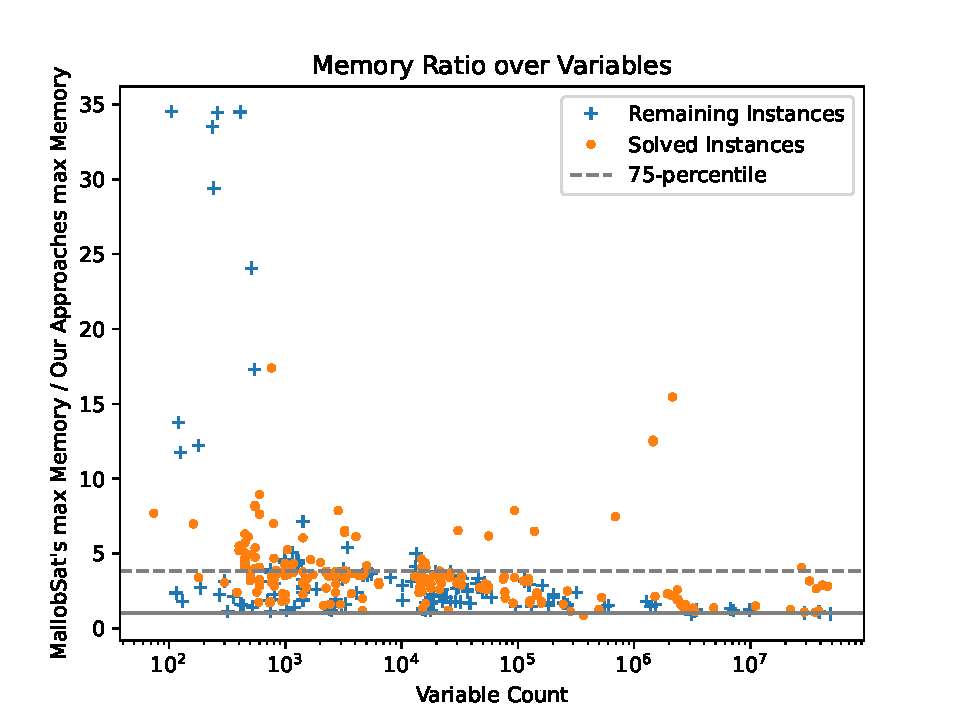
\includegraphics[scale=.45]{plots/1node_compare/mem_ratio_over_vars.pdf}
    \caption{1 node}
    \label{fig:memRatiosVars1node}
  \end{subfigure}
  \begin{subfigure}[c]{.45\textwidth}
    \center
    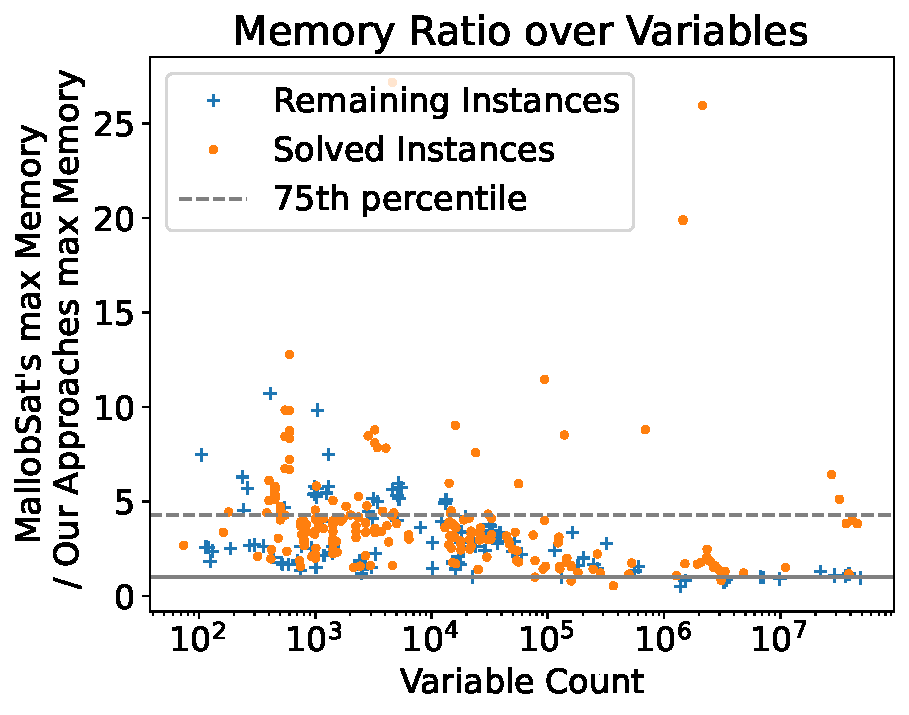
\includegraphics[scale=.45]{plots/4node_compare/mem_ratio_over_vars.pdf}
    \caption{4 nodes}
    \label{fig:memRatiosVars4node}
  \end{subfigure}
  \begin{subfigure}[c]{.45\textwidth}
    \center
    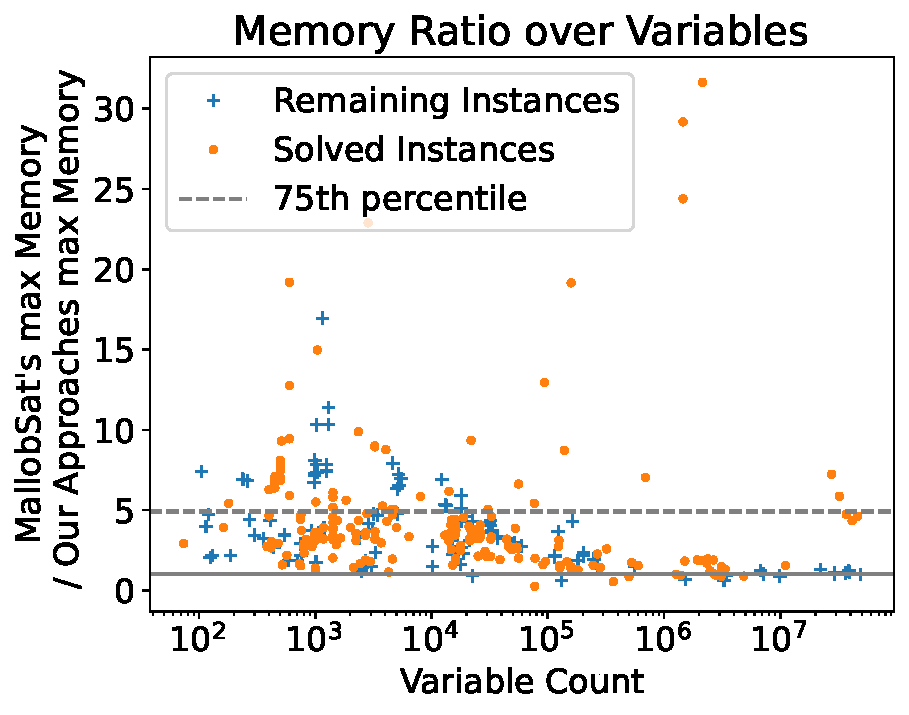
\includegraphics[scale=.45]{plots/16node_compare/mem_ratio_over_vars.pdf}
    \caption{16 nodes}
    \label{fig:memRatiosVars16node}
  \end{subfigure}
  \caption{Memory ratios between MallobSat and our approach. Each data point corresponds to a benchmark instance. TODO: eliminate + behind .}
  \label{fig:memRatiosVars}
\end{figure}

\begin{table}
  \center
  \begin{tabular}{ ccc }
    \toprule
    \#nodes & \#cores & 75th percentile \\
    \midrule
    1  & 48  & 3.864\\
    4  & 192 & 4.288\\
    16 & 762 & 4.916\\
    \bottomrule
  \end{tabular}
  \caption{Exact values of the 75th percentile for the ratios of peak memory consumption between MallobSat and our approach, as described in section \ref{sec:peakMemRatios}}
  \label{tab:memRatioPercentiles}
\end{table}

\label{sec:GMs}
Up to this point, we have only discussed peak memory consumption. We now take a closer look at the relative memory consumption of our approach throughout the course of calculation. To give an overview, we calculated the relative memory consumption between MallobSat and our approach for each second, that both solvers were active. For example, if MallobSat finished its execution after 30s and our algorithm finished after 35s, we calculated the ratio between MallobSat's memory consumption and our approach's memory consumption for every second of the first 30 seconds. This way, we only compare their memory consumption during runtime. Figure \ref{fig:memGmVars} shows the geometric means of these calculated ratios. We mark the geometric mean of all data points with a black line. The exact geometric means for each subplot are given in Table \ref{tab:memGM}.
We clearly see that all data points are well below one -- showing that our approach uses less (geometric mean) memory than MallobSat during the same runtime. We also observe that the densest areas, across all configurations, are around the respective geometric means of all data points. These geometric means shrink slightly with the number of used cores: from 0.282 for 48 nodes, over 0.256 for 192, and down to 0.216 for our maximum of 762 nodes.
All instances above $10^7$ variables encode so-called \textit{miters}. Miters encode two circuits to prove or disprove their equivalence via SAT solvers. We observe for all 14 of these fairly big instances that our approach's relative memory consumption, in relation to MallobSat, is noticeable shrinking with increasing numbers of cores.

% There are two instances on the top right, where our approach does not have a big advantage. No parallel sover solved these instances while serial Kissat solved them fairly easily...
% Names: oisc-subrv-sll-nested-13.cnf, oisc-subrv-sll-nested-11.cnf

\begin{figure}
  \center
  \begin{subfigure}[c]{.45\textwidth}
    \center
    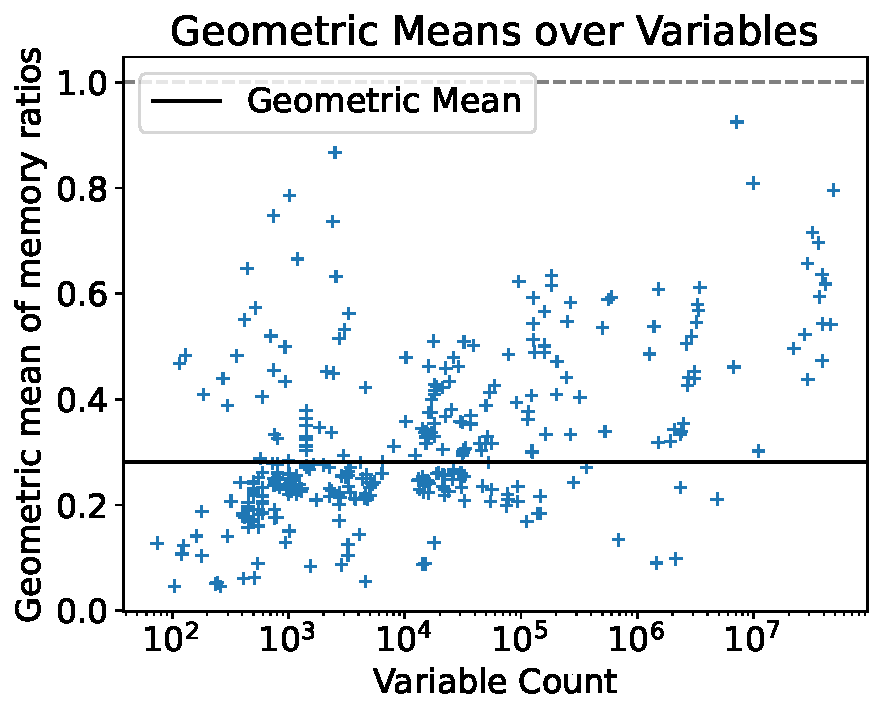
\includegraphics[scale=.45]{plots/1node_compare/mem_gm_over_vars.pdf}
    \caption{1 node}
  \end{subfigure}
  \begin{subfigure}[c]{.45\textwidth}
    \center
    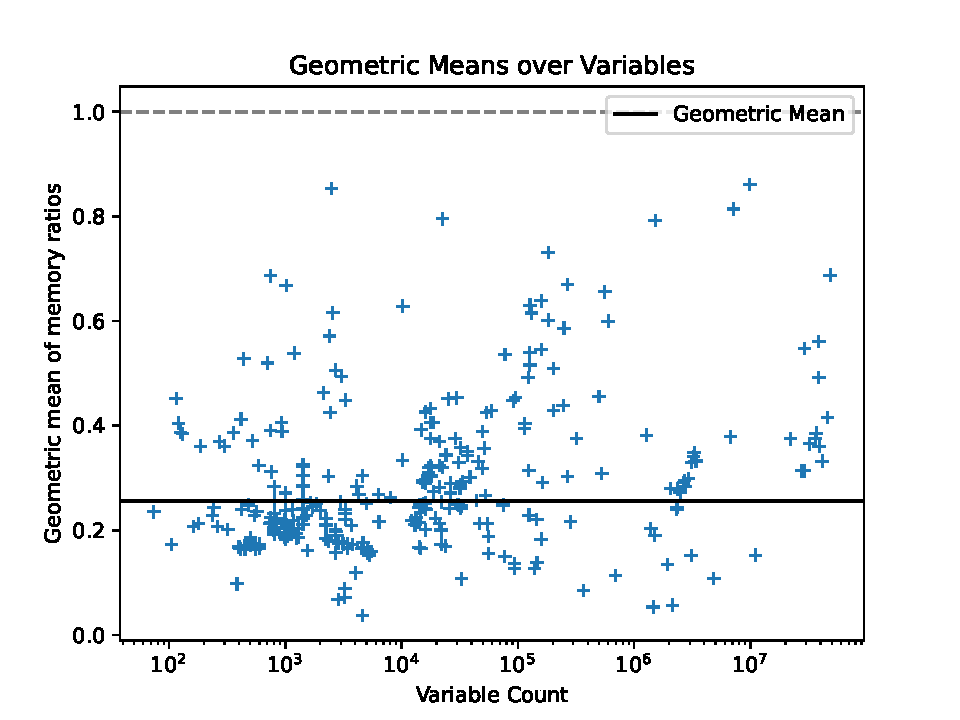
\includegraphics[scale=.45]{plots/4node_compare/mem_gm_over_vars.pdf}
    \caption{4 nodes}
  \end{subfigure}
  \begin{subfigure}[c]{.45\textwidth}
    \center
    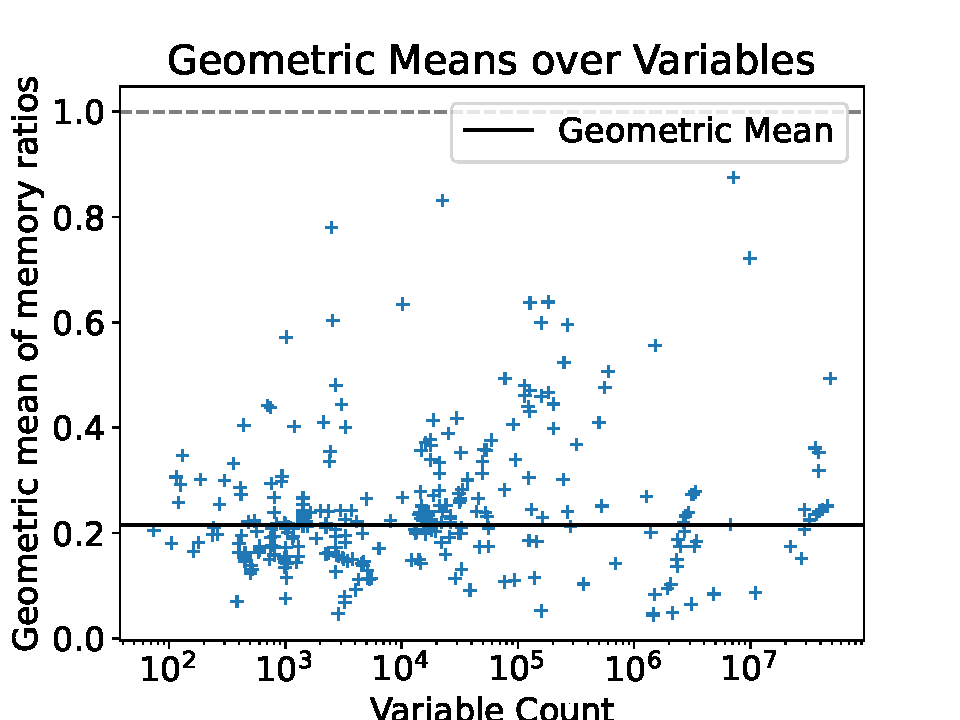
\includegraphics[scale=.45]{plots/16node_compare/mem_gm_over_vars.pdf}
    \caption{16 nodes}
  \end{subfigure}
  \caption{Geometric means for memory ratios between MallobSat and our approach per second. Each data point corresponds to a benchmark instance.}
  \label{fig:memGmVars}
\end{figure}

\begin{table}
  \center
  \begin{tabular}{ ccc }
    \toprule
    \#nodes & \#cores & Geometric Mean \\
    \midrule
    1  & 48  & 0.282\\
    4  & 192 & 0.256\\
    16 & 762 & 0.216\\
    \bottomrule
  \end{tabular}
  \caption{Geometric Means of the data points in Figure \ref{fig:memGmVars}. Calculated as described in section \ref{sec:GMs}.}
  \label{tab:memGM}
\end{table}

Figure \ref{fig:memRatiosSecs} shows the ratios between MallobSat and our approach per second, for all benchmark instances that reached the timeout of $300\,$s (both with MallobSat and our approach). The lines are smoothed, using a sliding window of five seconds and calculating its geometric mean.
First of all, we observe that for almost all instances the lines stay below a ratio of one. This indicates a systematic reduction in memory consumption for our approach, in comparison to MallobSat, during all stages of solving.
The second observation are the extreme jitters in some of our lines -- especially in the first few seconds of execution. We can explain this with a fairly simple effect of the search-only setting in our approach: At the beginning of the execution, we start a preprocessing thread in addition to the regular solving threads. This thread solely executes the preprocessing techniques implemented in Kissat. After the preprocessing is finished, the solver threads that are already running on the unprocessed instance, are gradually replaced by threads solving the preprocessed version of the problem formula. Since we collect a memory status every second, it is possible get measurements while a thread is being restarted. An offset of one second between the two compared solvers, results in an extreme discrepancy in memory consumption -- thus causing the extreme jitters in our plots.

\begin{figure}
  \center
  \begin{subfigure}[c]{.45\textwidth}
    \center
    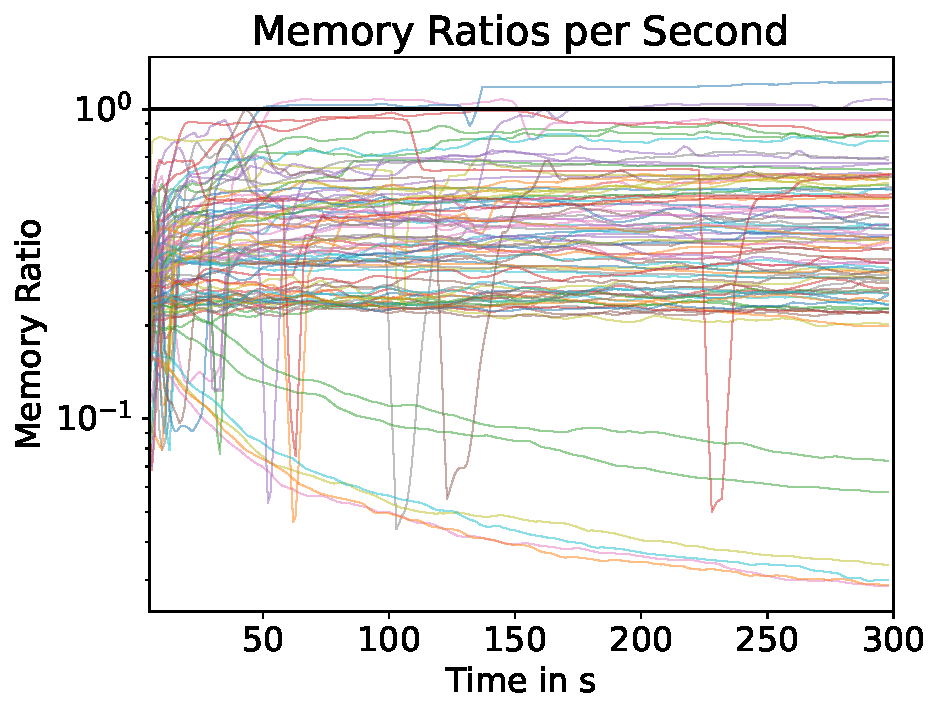
\includegraphics[scale=.45]{plots/1node_compare/mem_ratio_per_second.pdf}
    \caption{1 node}
  \end{subfigure}
  \begin{subfigure}[c]{.45\textwidth}
    \center
    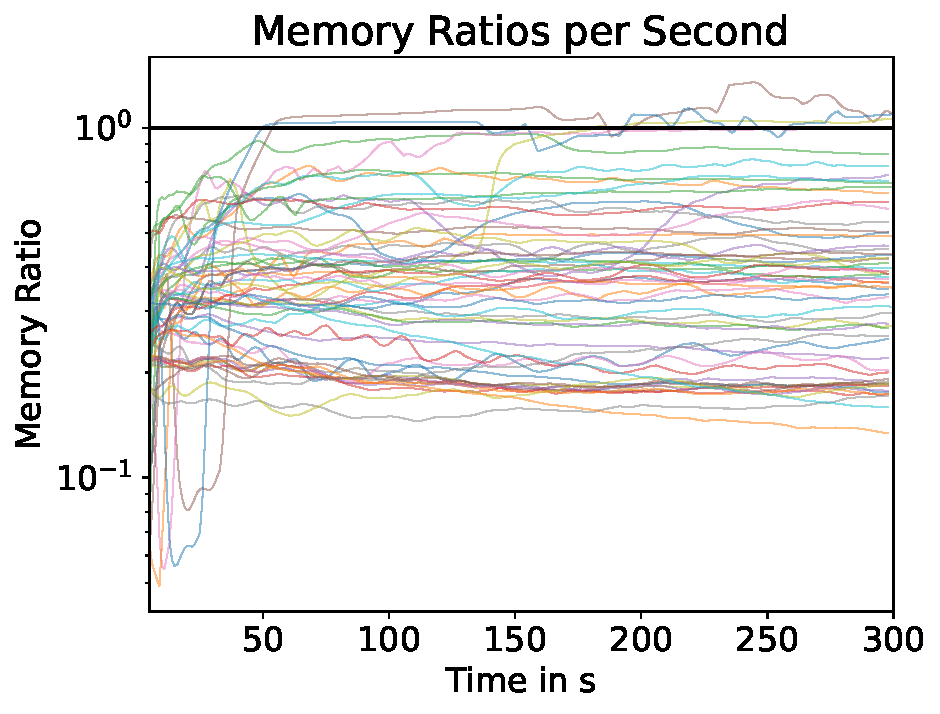
\includegraphics[scale=.45]{plots/4node_compare/mem_ratio_per_second.pdf}
    \caption{4 nodes}
  \end{subfigure}
  \begin{subfigure}[c]{.45\textwidth}
    \center
    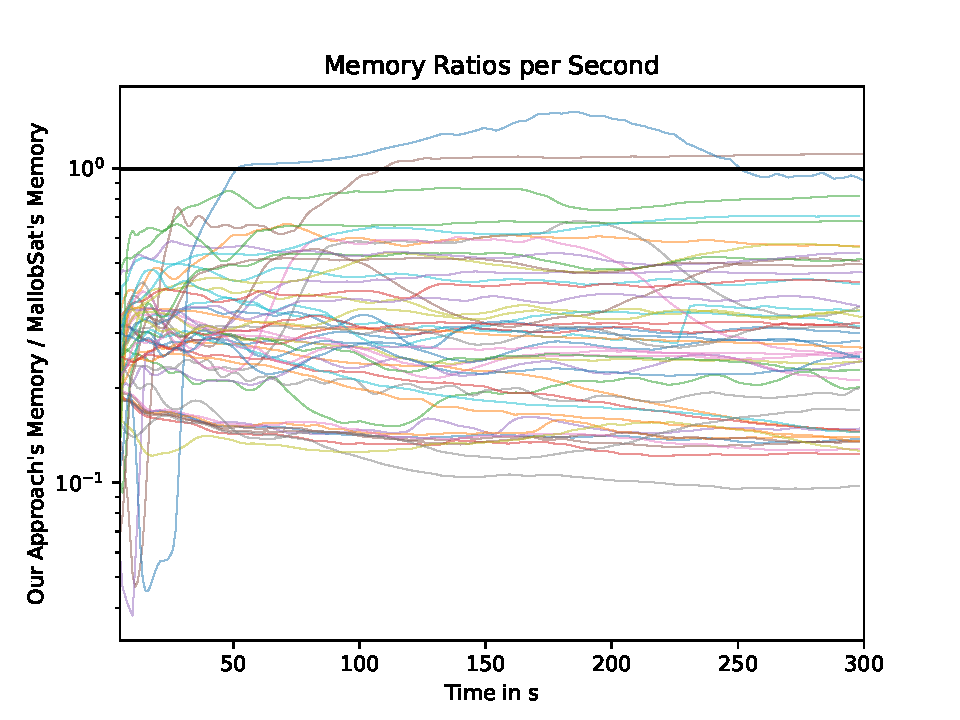
\includegraphics[scale=.45]{plots/16node_compare/mem_ratio_per_second.pdf}
    \caption{16 nodes}
  \end{subfigure}
  \caption{Memory ratios per second for all instances that reached the timeout of $300\,$s (both with MallobSat and our approach). The lines were smoothed, using a sliding window of size five seconds and calculating its geometric mean.}
  \label{fig:memRatiosSecs}
\end{figure}

% PAR-2 scores
% 1node_kis PAR-2: 180.82767644332498
% 1node_1p_48t PAR-2: 234.1985425415617
% 2node_1p_48t PAR-2: 210.472996790932
% 4node_kis PAR-2: 138.579572395466
% 4node_1p_48t PAR-2: 195.10140574811084
% 8node_1p_48t PAR-2: 184.21757448110833
% 16node_kis PAR-2: 114.08647329722923
% 16node_1p_48t PAR-2: 176.12921210075567
% Serial PAR-2: 1159.7390428211588

%%%%%%%%%%%%%%%%%%%%%%%%%%%%%%%%%%%%%%%%%%%%%%%%%%%%%%%%%%%%%%%%%%%%%%

\section{Conclusion}

Our approach cannot compare to MallobSat's scalability. MallobSat consistently solves more instances on the same number of cores. On 16 nodes (768 cores), MallobSat solved 28 instances more and achieved a geometric mean speedup of 20.073, compared to our geometric mean speedup of 10.26. We do, however, see a consistent improvement in runtime with increasing numbers of cores in our approach -- especially on more complex instances. This is also reflected in the geometric mean speedups, which grow with the number of cores. The differences become especially apparent for unsatisfiable instances. MallobSat solved 27 unsatisfiable instances that our approach could not solve, while our approach solved only one unsatisfiable instance that MallobSat could not.

Our approach does succeed in its goal to reduce memory consumption. In Section \ref{sec:compare}, we discuss a reduction in memory consumption per instance -- both solved and unsolved. We also show direct comparisons between the memory usage of our approach and that of MallobSat, both in absolute and relative values. Table \ref{tab:memGM} shows the geometric mean of the ratios between MallobSat's memory consumption and that of our approach, ranging from 0.216 to 0.282 -- depending on the number of cores used. The geometric mean of all these geometric means evaluates to 0.25. While this value alone cannot encapsulate the full complexity of our memory efficiency, it indicates an overall improvement in memory efficiency when compared to MallobSat. Furthermore, Figure \ref{fig:memRatiosSecs} shows that our improved memory efficiency does not only apply to maximum memory peaks, but also throughout all stages of solving.

Table \ref{tab:solvedPerGB} shows both the ratio of solved instances per overall memory used, and the ratio of solved instances per memory usage normalized by the number of cores. While MallobSat solves between 4.256 and 5.036 instances per GB of memory per core, our approach solves between 7.140 and 7.780.

\begin{table}
  \center
  \begin{tabular}{ cccccc }
    \toprule
    \multicolumn{2}{c}{Setup} & \multicolumn{2}{c}{Overall Used Memory} & \multicolumn{2}{c}{Normalized}\\
    \#nodes & \#cores & Our Approach & MallobSat & Our Approach & MallobSat \\
    \midrule
    1  & 48  & 0.149 & 0.089 & 7.140 & 4.256\\
    2  & 96  & 0.076 & -     & 7.306 & -\\
    4  & 192 & 0.039 & 0.026 & 7.583 & 5.036\\
    8  & 384 & 0.020 & -     & 7.780 & -\\
    16 & 762 & 0.010 & 0.006 & 7.766 & 4.924\\
    \bottomrule
  \end{tabular}
  \caption{Solved instances per GB of overall used memory in the middle and the same values normalized by the number of cores}
  \label{tab:solvedPerGB}
\end{table}

We thus conclude that our approach is applicable if memory efficiency per core is a greater concern than overall runtime. 

\subsection{Future Work}

In the future, we would like to extend our experiments to comprise more complex portfolios. This might result in a happy middle ground between MallobSat's scalability and our memory efficiency. We would also be interested in finding previously unsolved SAT problems with notoriously high memory demands and seeing whether we can solve them, given enough time.

%%%%%%%%%%%%%%%%%%%%%%%%%%%%%%%%%%%%%%%%%%%%%%%%%%%%%%%%%%%%%%%%%%%%%%

\clearpage

%%%%%%%%%%%%%%%%%%%%%%%%%%%%%%%%%%%%%%%%%%%%%%%%%%%%%%%%%%%%%%%%%%%%%%

\appendix

\section{Speedups per Family and Setup}
\label{app:speedupsFamiliesComplete}

\begin{longtable}{ lccccccc }
  \toprule
  family	&	\#	&	1node	&	2node	&	4node	&	8node	&	16node\\
  \midrule
  subset-cardinality	&	1	&	-	&	-	&	-	&	-	&	-\\
  waerden	&	1	&	-	&	-	&	-	&	-	&	-\\
  hardware-model-checking	&	1	&	-	&	-	&	-	&	-	&	-\\
  hgen	&	1	&	-	&	18.571	&	27.087	&	1130.439	&	1080.571\\
  coloring	&	8	&	-	&	-	&	-	&	-	&	-\\
  knights-problem	&	1	&	-	&	-	&	-	&	-	&	-\\
  risc-instruction-removal-subrv	&	2	&	-	&	-	&	-	&	-	&	-\\
  cril-misc	&	2	&	-	&	2.482	&	2.258	&	2.552	&	2.47\\
  relativized-pigeon-hole	&	2	&	-	&	-	&	-	&	-	&	-\\
  hamiltonian-cycle	&	1	&	-	&	-	&	8.508	&	9.305	&	9.424\\
  fermat	&	1	&	-	&	-	&	-	&	-	&	-\\
  binary-tree-parity	&	2	&	-	&	-	&	-	&	-	&	-\\
  sgen	&	2	&	-	&	-	&	-	&	-	&	-\\
  binary-pigeon-hole	&	1	&	-	&	-	&	-	&	-	&	-\\
  clique-width	&	1	&	-	&	-	&	-	&	-	&	-\\
  heule-folkman	&	11	&	0.425	&	-	&	0.416	&	0.449	&	0.444\\
  hypertree-decomposition	&	1	&	-	&	-	&	-	&	-	&	-\\
  cryptography-simon	&	10	&	0.221	&	0.234	&	0.227	&	0.2	&	0.18	\\
  subgraph-isomorphism	&	4	&	1.196	&	1.669	&	1.844	&	1.93	&	1.851	\\
  puzzle	&	1	&	1.604	&	1.767	&	1.78	&	1.85	&	1.95	\\
  miter	&	47	&	1.705	&	1.835	&	1.997	&	2.25	&	2.013	\\
  st-connectivity-principle	&	2	&	1.586	&	1.592	&	2.425	&	2.598	&	2.44	\\
  automata-synchronization	&	1	&	2.628	&	3.149	&	3.254	&	3.37	&	3.271	\\
  random-circuits	&	15	&	2.598	&	3.095	&	3.527	&	3.849	&	3.839	\\
  clique-formulas	&	1	&	3.246	&	3.364	&	3.772	&	4.142	&	3.748	\\
  cellular-automata	&	2	&	2.938	&	3.529	&	3.836	&	4.271	&	4.208	\\
  graph-isomorphism	&	1	&	3.538	&	3.791	&	3.476	&	4.226	&	3.88	\\
  planning	&	6	&	2.567	&	3.977	&	4.168	&	4.623	&	4.835	\\
  bitvector	&	4	&	3.391	&	3.788	&	3.984	&	4.55	&	4.813	\\
  software-verification	&	15	&	2.564	&	5.073	&	4.248	&	4.57	&	4.71	\\
  stedman-triples	&	2	&	3.926	&	2.783	&	3.821	&	7.486	&	4.85	\\
  tseitin-formulas	&	8	&	4.442	&	4.567	&	5.177	&	5.275	&	5.49	\\
  hardware-verification	&	5	&	4.621	&	5.369	&	5.556	&	6.036	&	6.161	\\
  summle	&	3	&	3.014	&	5.851	&	6.863	&	7.176	&	7.739	\\
  equivalence-chain-principle	&	4	&	4.16	&	5.462	&	6.263	&	6.88	&	7.626	\\
  erdos-discrepancy	&	1	&	4.25	&	4.83	&	6.517	&	7.707	&	7.387	\\
  random-modularity	&	1	&	6.073	&	3.31	&	5.157	&	11.028	&	6.742	\\
  or\_randxor	&	1	&	5.508	&	6.23	&	7.48	&	7.253	&	7.396	\\
  mutilated-chessboard	&	3	&	5.353	&	5.276	&	7.803	&	8.323	&	9.425	\\
  scheduling	&	50	&	5.333	&	6.434	&	7.944	&	8.384	&	8.799	\\
  rooks	&	3	&	6.83	&	8.56	&	6.281	&	7.858	&	7.899	\\
  grs-fp-comm	&	2	&	6.942	&	7.939	&	9.583	&	10.425	&	10.679	\\
  heule-nol	&	11	&	5.988	&	11.793	&	7.786	&	10.231	&	12.876	\\
  cryptography-ascon	&	6	&	7.396	&	8.273	&	10.115	&	8.709	&	14.008	\\
  popularity-similarity	&	1	&	10.297	&	10.371	&	10.352	&	10.474	&	10.816	\\
  maxsat-optimum	&	13	&	7.419	&	7.32	&	12.362	&	13.762	&	14.899	\\
  quantum-kochen-specker	&	10	&	9.356	&	11.237	&	11.186	&	11.137	&	11.005	\\
  reg-n	&	4	&	0.549	&	28.761	&	26.837	&	26.765	&	27.78	\\
  cryptography	&	7	&	6.32	&	16.922	&	9.289	&	21.402	&	23.632	\\
  quasigroup-completion	&	2	&	8.779	&	6.998	&	12.279	&	30.304	&	32.551	\\
  hamiltonian	&	40	&	8.968	&	14.409	&	19.398	&	23.315	&	26.351	\\
  argumentation	&	21	&	13.01	&	16.268	&	18.577	&	21.941	&	20.716	\\
  battleship	&	1	&	7.976	&	11.49	&	22.608	&	38.895	&	28.755	\\
  ramsey	&	1	&	19.718	&	18.278	&	18.859	&	19.927	&	19.178	\\
  independent-set	&	15	&	16.442	&	18.038	&	20.981	&	27.173	&	25.9	\\
  pythagorean-triples	&	1	&	4.46	&	23.726	&	24.031	&	96.261	&	28.008	\\
  crafted-cec	&	1	&	28.769	&	28.202	&	30.506	&	34.541	&	45.252	\\
  polynomial-multiplication	&	4	&	25.567	&	34.021	&	22.424	&	24.579	&	121.641	\\
  minimum-disagreement-parity	&	17	&	40.311	&	22.119	&	24.766	&	46.884	&	58.316	\\
  random-csp	&	2	&	14.849	&	31.507	&	32.744	&	71.948	&	98.142	\\
  unknown	&	1	&	87.088	&	29.251	&	89.022	&	103.831	&	120.212	\\
  circuit-multiplier	&	1	&	90.994	&	105.262	&	33.202	&	82.974	&	264.479	\\
  influence-maximization	&	1	&	41.459	&	96.668	&	43.252	&	145.409	&	279.558	\\
  rbsat	&	5	&	47.606	&	64.654	&	76.039	&	186.204	&	221.286	\\
  tree-decomposition	&	1	&	97.594	&	73.685	&	70.701	&	174.601	&	485.546	\\
  \bottomrule
  \caption{Speedups per family and Solver Setup}
  \label{tab:speedupsFamiliesComplete}
\end{longtable}

\section{PAR-2 Scores}

We evaluated the \textit{penalized average runtime (PAR-2)} score, as it was used in the SAT competition \cite{satCompWebsite} of 2024 to evaluate submitted solvers. It is calculated by taking the weighted average runtime over all instances, with unsolved instances included at a penalty of twice the time limit. The PAR-2 scores for MallobSat and our approach, for our time limit of 300 seconds, are listed in Table \ref{tab:par2}. They are, however, not directly comparable to the results of the SAT competition, since the competition used a much larger time limit of 5000 seconds.

\begin{table}[h]
  \center
  \begin{tabular}{ cccccc }
    \toprule
    \#nodes & \#cores & Our Algorithm & MallobSat\\
    \midrule
    1  & 48  & 234.199 & 180.828\\
    2  & 96  & 210.472 & -\\
    4  & 192 & 195.101 & 138.580\\
    8  & 384 & 184.218 & -\\
    16 & 762 & 176.129 & 114.086\\
    \bottomrule
  \end{tabular}
  \caption{PAR-2 scores for a time limit of 300 seconds.}
  \label{tab:par2}
\end{table}

\section{LBDs in Clause sharing}

Schreiber et al. \cite{searchOnlyPaper} found LBDs to be an impractical metric for clause sharing operations. They support this claim, in part, by running MallobSat with artificial LBDs for shared clauses. More precisely, the LBDs are either set to the maximum (i.e., the clause length) or drawn from a random distribution (uniform or triangular). They find, setting the LBDs to their maximum for every clause performs similar to the original LBDs. Both the uniform and triangular distributions perform slightly worse.

We were able to reproduce these findings, with our configuration, that runs only Gimsatul as solver engines in MallobSat. This further strengthens the notion that LBDs do not constitute a meaningful metric when deciding which clauses to share.

\bibliographystyle{eptcs}
\bibliography{literatur}

\end{document}
